% Options for packages loaded elsewhere
\PassOptionsToPackage{unicode}{hyperref}
\PassOptionsToPackage{hyphens}{url}
%
\documentclass[
  man]{apa6}
\usepackage{amsmath,amssymb}
\usepackage{lmodern}
\usepackage{iftex}
\ifPDFTeX
  \usepackage[T1]{fontenc}
  \usepackage[utf8]{inputenc}
  \usepackage{textcomp} % provide euro and other symbols
\else % if luatex or xetex
  \usepackage{unicode-math}
  \defaultfontfeatures{Scale=MatchLowercase}
  \defaultfontfeatures[\rmfamily]{Ligatures=TeX,Scale=1}
  \setmainfont[]{Arial}
\fi
% Use upquote if available, for straight quotes in verbatim environments
\IfFileExists{upquote.sty}{\usepackage{upquote}}{}
\IfFileExists{microtype.sty}{% use microtype if available
  \usepackage[]{microtype}
  \UseMicrotypeSet[protrusion]{basicmath} % disable protrusion for tt fonts
}{}
\makeatletter
\@ifundefined{KOMAClassName}{% if non-KOMA class
  \IfFileExists{parskip.sty}{%
    \usepackage{parskip}
  }{% else
    \setlength{\parindent}{0pt}
    \setlength{\parskip}{6pt plus 2pt minus 1pt}}
}{% if KOMA class
  \KOMAoptions{parskip=half}}
\makeatother
\usepackage{xcolor}
\usepackage{graphicx}
\makeatletter
\def\maxwidth{\ifdim\Gin@nat@width>\linewidth\linewidth\else\Gin@nat@width\fi}
\def\maxheight{\ifdim\Gin@nat@height>\textheight\textheight\else\Gin@nat@height\fi}
\makeatother
% Scale images if necessary, so that they will not overflow the page
% margins by default, and it is still possible to overwrite the defaults
% using explicit options in \includegraphics[width, height, ...]{}
\setkeys{Gin}{width=\maxwidth,height=\maxheight,keepaspectratio}
% Set default figure placement to htbp
\makeatletter
\def\fps@figure{htbp}
\makeatother
\setlength{\emergencystretch}{3em} % prevent overfull lines
\providecommand{\tightlist}{%
  \setlength{\itemsep}{0pt}\setlength{\parskip}{0pt}}
\setcounter{secnumdepth}{-\maxdimen} % remove section numbering
% Make \paragraph and \subparagraph free-standing
\ifx\paragraph\undefined\else
  \let\oldparagraph\paragraph
  \renewcommand{\paragraph}[1]{\oldparagraph{#1}\mbox{}}
\fi
\ifx\subparagraph\undefined\else
  \let\oldsubparagraph\subparagraph
  \renewcommand{\subparagraph}[1]{\oldsubparagraph{#1}\mbox{}}
\fi
\newlength{\cslhangindent}
\setlength{\cslhangindent}{1.5em}
\newlength{\csllabelwidth}
\setlength{\csllabelwidth}{3em}
\newlength{\cslentryspacingunit} % times entry-spacing
\setlength{\cslentryspacingunit}{\parskip}
\newenvironment{CSLReferences}[2] % #1 hanging-ident, #2 entry spacing
 {% don't indent paragraphs
  \setlength{\parindent}{0pt}
  % turn on hanging indent if param 1 is 1
  \ifodd #1
  \let\oldpar\par
  \def\par{\hangindent=\cslhangindent\oldpar}
  \fi
  % set entry spacing
  \setlength{\parskip}{#2\cslentryspacingunit}
 }%
 {}
\usepackage{calc}
\newcommand{\CSLBlock}[1]{#1\hfill\break}
\newcommand{\CSLLeftMargin}[1]{\parbox[t]{\csllabelwidth}{#1}}
\newcommand{\CSLRightInline}[1]{\parbox[t]{\linewidth - \csllabelwidth}{#1}\break}
\newcommand{\CSLIndent}[1]{\hspace{\cslhangindent}#1}
\ifLuaTeX
\usepackage[bidi=basic]{babel}
\else
\usepackage[bidi=default]{babel}
\fi
\babelprovide[main,import]{english}
% get rid of language-specific shorthands (see #6817):
\let\LanguageShortHands\languageshorthands
\def\languageshorthands#1{}
% Manuscript styling
\usepackage{upgreek}
\captionsetup{font=singlespacing,justification=justified}

% Table formatting
\usepackage{longtable}
\usepackage{lscape}
% \usepackage[counterclockwise]{rotating}   % Landscape page setup for large tables
\usepackage{multirow}		% Table styling
\usepackage{tabularx}		% Control Column width
\usepackage[flushleft]{threeparttable}	% Allows for three part tables with a specified notes section
\usepackage{threeparttablex}            % Lets threeparttable work with longtable

% Create new environments so endfloat can handle them
% \newenvironment{ltable}
%   {\begin{landscape}\centering\begin{threeparttable}}
%   {\end{threeparttable}\end{landscape}}
\newenvironment{lltable}{\begin{landscape}\centering\begin{ThreePartTable}}{\end{ThreePartTable}\end{landscape}}

% Enables adjusting longtable caption width to table width
% Solution found at http://golatex.de/longtable-mit-caption-so-breit-wie-die-tabelle-t15767.html
\makeatletter
\newcommand\LastLTentrywidth{1em}
\newlength\longtablewidth
\setlength{\longtablewidth}{1in}
\newcommand{\getlongtablewidth}{\begingroup \ifcsname LT@\roman{LT@tables}\endcsname \global\longtablewidth=0pt \renewcommand{\LT@entry}[2]{\global\advance\longtablewidth by ##2\relax\gdef\LastLTentrywidth{##2}}\@nameuse{LT@\roman{LT@tables}} \fi \endgroup}

% \setlength{\parindent}{0.5in}
% \setlength{\parskip}{0pt plus 0pt minus 0pt}

% Overwrite redefinition of paragraph and subparagraph by the default LaTeX template
% See https://github.com/crsh/papaja/issues/292
\makeatletter
\renewcommand{\paragraph}{\@startsection{paragraph}{4}{\parindent}%
  {0\baselineskip \@plus 0.2ex \@minus 0.2ex}%
  {-1em}%
  {\normalfont\normalsize\bfseries\itshape\typesectitle}}

\renewcommand{\subparagraph}[1]{\@startsection{subparagraph}{5}{1em}%
  {0\baselineskip \@plus 0.2ex \@minus 0.2ex}%
  {-\z@\relax}%
  {\normalfont\normalsize\itshape\hspace{\parindent}{#1}\textit{\addperi}}{\relax}}
\makeatother

% \usepackage{etoolbox}
\makeatletter
\patchcmd{\HyOrg@maketitle}
  {\section{\normalfont\normalsize\abstractname}}
  {\section*{\normalfont\normalsize\abstractname}}
  {}{\typeout{Failed to patch abstract.}}
\patchcmd{\HyOrg@maketitle}
  {\section{\protect\normalfont{\@title}}}
  {\section*{\protect\normalfont{\@title}}}
  {}{\typeout{Failed to patch title.}}
\makeatother

\usepackage{xpatch}
\makeatletter
\xapptocmd\appendix
  {\xapptocmd\section
    {\addcontentsline{toc}{section}{\appendixname\ifoneappendix\else~\theappendix\fi\\: #1}}
    {}{\InnerPatchFailed}%
  }
{}{\PatchFailed}
\keywords{Locus of Control; Classical Test Theory; Item Response Theory; Exploratory Factor Analysis; Confirmatory Factor Analysis; Convergent validity\newline\indent Word count: 4962}
\DeclareDelayedFloatFlavor{ThreePartTable}{table}
\DeclareDelayedFloatFlavor{lltable}{table}
\DeclareDelayedFloatFlavor*{longtable}{table}
\makeatletter
\renewcommand{\efloat@iwrite}[1]{\immediate\expandafter\protected@write\csname efloat@post#1\endcsname{}}
\makeatother
\usepackage{lineno}

\linenumbers
\usepackage{csquotes}
\ifLuaTeX
  \usepackage{selnolig}  % disable illegal ligatures
\fi
\IfFileExists{bookmark.sty}{\usepackage{bookmark}}{\usepackage{hyperref}}
\IfFileExists{xurl.sty}{\usepackage{xurl}}{} % add URL line breaks if available
\urlstyle{same} % disable monospaced font for URLs
\hypersetup{
  pdftitle={Psychometric Evaluation and Validation of Bangla Rotter Internal-External Scale with Classical Test Theory and Item Response theory},
  pdfauthor={Mushfiqul Anwar Siraji1 \& Shamsul Haque1},
  pdflang={en-EN},
  pdfkeywords={Locus of Control; Classical Test Theory; Item Response Theory; Exploratory Factor Analysis; Confirmatory Factor Analysis; Convergent validity},
  hidelinks,
  pdfcreator={LaTeX via pandoc}}

\title{Psychometric Evaluation and Validation of Bangla Rotter Internal-External Scale with Classical Test Theory and Item Response theory}
\author{Mushfiqul Anwar Siraji\textsuperscript{1} \& Shamsul Haque\textsuperscript{1}}
\date{}


\shorttitle{Bangla Rotter's I-E Scale}

\authornote{

Mushfiqul Anwar Siraji \url{https://orcid.org/0000-0003-0127-9982}

Shamsul Haque \url{https://orcid.org/0000-0002-1561-6989}

We have preregistered this study's design and analysis plan in Open Science Framework (Preregistration DOI: 10.17605/OSF.IO/9KT87) and can be accessed at \url{https://osf.io/9kt87}. All data, analysis code underlying this article and a Rmarkdown reproducible manuscript have been made publicly available at GitHub and can be accessed at \url{https://github.com/masiraji/Rotter-I-E-Scale}.

The authors made the following contributions. Mushfiqul Anwar Siraji: Conceptualization, Writing - Original Draft Preparation, Writing - Review \& Editing; Shamsul Haque: Conceptualization, Writing - Review \& Editing.

Correspondence concerning this article should be addressed to Shamsul Haque, Monash University Malaysia,Jalan Lagoon Selatan, 47500 Bandar Sunway,Selangor Darul Ehsan, Malaysia.. E-mail: \href{mailto:shamsul@monash.edu}{\nolinkurl{shamsul@monash.edu}}

}

\affiliation{\vspace{0.5cm}\textsuperscript{1} Monash University, Malaysia}

\abstract{%
There is no psychometric tool to assess locus of control for Bangla-speaking people. Hence, we attempted to translate the 23-item Rotter's Internal-External scale into Bangla and validate it on Bangladeshi adult participants. In Study 1 (N = 300), we translated the items into Bangla and conducted an exploratory factor analysis, which revealed a one-factor solution with 12 items. In Study 2 (N =178) confirmatory factor analysis yielded the best fit with 11 items (CFI =.98, TLI = .97, RMSEA = .00). Reliability coefficient of this 11-item scale was satisfactory (McDonald's Omega = .72). The scale's significant correlations with Internal Control Index (a locus of control scale), Neuroticism and Openness to Experience from Big Five Personality Inventory demonstrated its convergent validity. The item quality was assessed on the combined samples of Study 1 \& 2 (N=478) using the item response theory (IRT), which showed that the scale was composed of easy, moderate, and hard items. Item discrimination analysis indicated sufficient discriminating power of the items (.49 to 2.21). Test information curve showed the scale's ability to discriminate between external and internal locus of control. These psychometric properties indicate the usability of the Bangla version of Rotter's Internal-External scale.
}



\begin{document}
\maketitle

\hypertarget{introduction}{%
\section{Introduction}\label{introduction}}

Locus of Control (LoC) is the individual's belief about the contingency of the outcome of an event on their internal qualities and behavior vs.~other external attributes like chance or fate (J. B. Rotter, 1966). LoC influences a broad spectrum of situations closely related to achievement, success and learning. The LoC can be viewed as a bipolar continuum ranging from internal to external, indicating an individual's disposition on the reinforcement expectancy. Social learning theory suggests human behavior is lead by reinforcement and the belief regarding the dependency of the reinforcement on an individual's ability and action (Bandura \& Walters, 1977; Duttweiler, 1984).Individuals with internal LoC believe the reinforcement and fundamental control over the event's outcome are contingent on their ability, behavior and efforts. However, for the individuals with external LoC, the fundamental sense of agency of life and reinforcement are bestowed on the attributes like fate, luck, change or other powerful entities (Marsh \& Richards, 1987; J. B. Rotter, 1966; Julian B. Rotter, Chance, \& Phares, 1972).

Since J. B. Rotter (1966) introduced the term LoC, it has been widely used to understand people's behavior in different domains, including academic achievement (Findley \& Cooper, 1983; Karaman, Nelson, \& Cavazos Vela, 2018), health (Jacobs-Lawson, Waddell, \& Webb, 2011), professional competence(Mantesso, Petrucka, \& Bassendowski, 2008; Smidt, Kammermeyer, Roux, Theisen, \& Weber, 2018; Witt, 1988) and consumer behavior (Lee, Chang, Cheng, \& Chen, 2018; Rodriguez-Ricardo, Sicilia, \& López, 2019). Internal LoC is attributed to better health care management and self-assessment (Pourhoseinzadeh, Gheibizadeh, Moradikalboland, et al., 2017). Internal LoC also positively influences academic success (Karaman et al., 2018) . External LoC is associated with increased depression, anxiety, stress (Kurtović, Vuković, \& Gajić, 2018), and personality factors including high neuroticism (Horner, 1996) and low openness to experience (Kobasa, Maddi, \& Kahn, 1982; Sherman, Pelletier, \& Ryckman, 1973; Taylor, 1983, 1983). Assessment of LoC is also beneficial in the different therapeutic processes (E. K. Baker, 1979; Delsignore \& Schnyder, 2007). Individuals with internal LoC are more receptive to information (Cavaiola \& Strohmetz, 2009), more resilient and hopeful than external LoC, thus facilitating the favorable outcome in the psychotherapy (Foon, 1987).LoC also facilitates the ``Transactional Analysis'' based counselling process by indicating an individual's predominant ego-states (Loffredo, 1998). Internal LoC is associated with ``Adult'' ego state and External LoC is associated with ``Adapted Child'' ego state (Loffredo, 1998).

Rotter's Internal-External (I-E) (J. B. Rotter, 1966) scale is the most widely used scale to measure the LoC of an individual. However, the origin of this scale is from an individualist society (Hofstede, 1984; Smith, Trompenaars, \& Dugan, 1995). Members of individualist culture define their identity by personal life choices, whereas members of collectivist countries emphasize the membership of groups (Hofstede, 1984). Smith et al. (1995) coined some fundamental problems of using Rotter's I-E scale in collectivist cultures, including 'modesty bias'', where individuals may guide their responses to represent the group's opinion instead of individual preference. Also values parallel to LoC including ``mastery over the environment'' and ``harmony with the environment'' are differentially endorsed by members of different cultures (Schwartz, 1990, 1992). This indicates the cultural susceptibility of the construct: LoC which may lead to different latent structures across various cultures. J. B. Rotter (1966) mentioned one general factor and several other but less essential factors and conferred the structure as unidimensional. However,studies in the USA (Joe \& Jahn, 1973; Mirels, 1970) and other countries (Marsh \& Richards, 1987; Niles, 1981; Tobacyk, 1978; Tyler, Dhawan, \& Sinha, 1989) have established the multidimensional nature of Rotter's I-E scale. Marsh and Richards (1987) summarized 20 studies which analyzed the latent structure by exploratory factor analysis(EFA). summarized 20 studies that analyzed the latent structure by exploratory factor analysis (EFA). They reported that the number of possible interpretable factors ranged between 2 to 6 with two recurring factors: ``political control''and ``personal control''. The emergence of ``political control'' and ``personal control'' as salient factors in Rotter's I-E Scale was first reported in the work of Mirels (1970). He conducted an EFA on 316 (f = 157) undergraduate students and reported these two factors. Items clustered under ``personal control'' stemmed from the individual's inclination to prefer personal ability and hard work over luck. The ``Political control'' factor focuses on the individual's disposition regarding their ability to control the political and world affairs as a part of the social system. Smith et al. (1995) administered the Rotter's I-E scale on 9140 participants from 43 different countries and reported three interpretable dimensions: ``personal-political'', ``individual-social'' and ``luck.'' They reported a trend of fatalism about political events and high preference on luck among the included Asian nations. However, Studies in the Netherlands (Andriessen \& Van Cadsand, 1983), Brazil (Nagelschmidt \& Jakob, 1977), Australia (Watson, 1981), Sri Lanka (Niles, 1981) reported only the ``personal control'' factor indicating the susceptibility of the latent construct structure of Rotter's I-E scale to cultural variation.

Due to this susceptibility, it is inappropriate to use the Rotter's I-E scale in Bangladesh without proper psychometric calibration. Besides, there is a dearth of psychometrically valid scales in Bangladesh to measure the LoC culturally sensitively. We conducted two studies involving Bangladeshi elementary school teachers to culturally adapt and psychometrically validate Rotter's I-E scale by following classical test theory (CTT) and item response theory (IRT). CTT uses a set of concepts (true score, observed score, reliability) and provides information on the whole scale (DeVellis, 2006). CTT attributes the observed scores obtained on a scale to the unobservable variable of interest and possible measurement errors. The reliability coefficients indicate how closely the observed score reflects the unobservable variable (DeVellis, 2006). IRT assesses the item quality across the different latent construct levels and complements the psychometric analysis by providing information regarding the item's ability to discriminate among the respondents across the latent construct continuum (Kazemi \& Kajonius, 2021). It also provides information on the level of latent construct a respondent requires to attain a 50\% chance to score towards the positive high construct direction for a particular item (Kazemi \& Kajonius, 2021). TOur first study culturally adapted the scale and identified the latent construct structure by exploratory factor analysis. The second study verified the latent construct structure that emerged in the first study by a confirmatory factor analysis. Subsequect psychometric propertise were also established using CTT and IRT.

\hypertarget{study-1-translations-and-factor-structure}{%
\section{Study 1: Translations and Factor Structure}\label{study-1-translations-and-factor-structure}}

Our first study had three objectives. First, to translate the items from the original language to the Bangla language in a culturally meaningful way. Second, to assess the content validity. Third, to conduct an exploratory factor analysis to understand the latent structure

\hypertarget{methods}{%
\subsection{Methods}\label{methods}}

\hypertarget{participants}{%
\subsection{Participants}\label{participants}}

A large group of 312 Bangladeshi adults participated in Study 1. Twelve participants were excluded due to incomplete data. For exploring initial factor structure, a sample of 250-300 is recommended (Comrey \& Lee, 1992; Schönbrodt \& Perugini, 2013) . Participants were recruited through email invitation following snowballing techniques. Out of 300 participants 108.67\% (326) were female ranging in age from 21 to 52 years (29.20±4.92) and 50.67\% (152) were male with an age range between 21 to 45 years (32.39±4.17). Average years of education for the females were 15.28±2.09 and for the males were 16.71±.0.94. 72\% of the participants were married.

\hypertarget{material}{%
\subsection{Material}\label{material}}

Rotter's Internal-External (I-E) scale consists of 23 item pairs in a forced-choice format with six additional filler pairs. Each pair contains one statement focusing on internal LoC and another focusing on external LoC. The score ranges from 0 to 23, with a higher score indicating higher external LoC. Internal consistency Kuder-Richardson coefficient was .69 in the original scale among the national stratified sample (Franklin, 1963).

\hypertarget{procedure}{%
\subsection{Procedure}\label{procedure}}

\hypertarget{data-collection}{%
\subsubsection{Data Collection}\label{data-collection}}

Invitation emails were sent to the potential participants with appropriate explanatory statements. Once the participants voluntarily agreed to participate, their consent was recorded digitally. The data collection commenced from June 2021 to July 2021

\hypertarget{scale-translation}{%
\subsubsection{Scale Translation}\label{scale-translation}}

We followed ICT (Bartram et al., 2018) guidelines to translate and adapt the scale. A robust literature review was conducted to ensure the construct equivalence of ``Locus of control'' to ensure cross-cultural applicability. Based on the reviewed literature, it was agreed that the construct is equivalent in meaning across ``Western'' and ``Bangladeshi'' cultures. Two bilingual researchers (PhD in Psychology) natives in Bangla translated the original version (English) to Bangla. The two translated version was then judged and synthesized by the authors. Subsequently, two bilingual researchers (One PhD, one MS in psychology) back-translated the Bangla scale into English with no knowledge of the original work. The authors synthesized the two back-translations and compared it with the original scale, and made necessary amendments.

\hypertarget{content-validity-expert-panel-review}{%
\subsubsection{Content Validity: Expert Panel Review}\label{content-validity-expert-panel-review}}

We gave the amended synthesized scale to 8 mental health professionals. They assessed the content validity of the scale (23 items) independently. They confirmed the relevance of the items using a 4-point Likert type scale (1: not at all relevant, 2: slightly relevant, 3: quite Relevant, 4: Highly Relevant). We estimated the item-level content validity (I-CVI) and scale-level content validity index (S-CVI). Any Item with an I-CVI score higher than 0.83 was retained (Lynn, 1986; Polit, Beck, \& Owen, 2007). Two items were below the cut-off values thus readjusted and analyzed again.The S-CVI was .94, estimated using the average method and indicated satisfactory content validity (Lynn, 1986; Polit et al., 2007).

\hypertarget{analytic-strategies}{%
\subsubsection{Analytic Strategies}\label{analytic-strategies}}

We used R (version 4.1.0), including R-packages ``Psych'' (R Core Team, 2021) and ``ggplot2''(Wickham, 2016), for our analyses. Since Rotter's I-E scale used a dichotomous forced choice and both univariate normality {[}TABLE \ref{tab:tabDes}{]} and multivariate normality assumptions are violated we performed the exploratory factor analysis using a tetrachoric correlation matrix (Watkins, 2020). We employed weighted least squares (WLS) as a factor extraction method to examine the latent construct structure. WLS is more robust towards violation of normality assumptions (Fabrigar, Wegener, MacCallum, \& Strahan, 1999). An orthogonal rotation technique: varimax was chosen following the literature investigating the latent structure of Rotter's I-E scale (Joe \& Jahn, 1973; Mirels, 1970; Tobacyk, 1978). Before the EFA, necessary assumptions, including sample adequacy, quality of correlation matrix were assessed. As the commonalities for each item found in the previous studies were not \textgreater.70 (Joe \& Jahn, 1973; Mirels, 1970; Tobacyk, 1978) , instead of relying on Kaiser criterion of eigenvalues greater than one, we relied on scree plot (Stevens, 2009) . We supplemented the scree plot (Cattell, 1966) with Horn's parallel analysis (Horn, 1965), minimum average partials method (Velicer, 1976), and hull method (Lorenzo-Seva, Timmerman, \& Kiers, 2011). We compared the root mean square of the residuals (RMSR) values obtained for the solutions to determine the best factor structure. \(RMSR \le .08\) is preferred (Brown, 2015). Additionally, to identify the simple structure we followed the following guidelines recommended by psychometricians (i) no factors with fewer than three items (ii) no factors with a factor loading \textless0.3 (iii) no items with cross-loading greater than .3 across factors (Bandalos \& Finney, 2018; Child, 2006; Mulaik, 2009; Watkins, 2020)

\hypertarget{result-and-discussion}{%
\subsection{Result and Discussion}\label{result-and-discussion}}

\hypertarget{sampling-adequacy}{%
\subsubsection{Sampling Adequacy}\label{sampling-adequacy}}

Sampling adequacy was investigated by Kaiser-Meyer-Olkin (KMO) measures of sampling adequacy (Kaiser, 1974). The overall KMO vale for 23 items was 0.68 which was above the cutoff value of .50 indicating a mediocre sample (Hutcheson, 1999).

\hypertarget{descriptive-statistics-and-item-analysis}{%
\subsubsection{Descriptive Statistics and Item Analysis}\label{descriptive-statistics-and-item-analysis}}

\begin{table}[tbp]

\begin{center}
\begin{threeparttable}

\caption{\label{tab:tabDes}Descriptive Statistics}

\begin{tabular}{lllllll}
\toprule
Items & \multicolumn{1}{c}{Mean} & \multicolumn{1}{c}{SD} & \multicolumn{1}{c}{Skew} & \multicolumn{1}{c}{Kurtosis} & \multicolumn{1}{c}{Normality} & \multicolumn{1}{c}{Corrected.item.total.correlation}\\
\midrule
item2 & 0.17 & 0.37 & 1.78 & 1.17 & 0.45* & 0.24\\
item3 & 0.87 & 0.34 & -2.15 & 2.62 & 0.40* & 0.13\\
item4 & 0.43 & 0.50 & 0.30 & -1.92 & 0.63* & 0.28\\
item5 & 0.14 & 0.34 & 2.10 & 2.44 & 0.41* & 0.25\\
item6 & 0.32 & 0.47 & 0.75 & -1.44 & 0.59* & 0.08\\
item7 & 0.85 & 0.35 & -1.99 & 1.96 & 0.42* & 0.23\\
item9 & 0.29 & 0.45 & 0.94 & -1.12 & 0.57* & 0.41\\
item10 & 0.08 & 0.28 & 3.00 & 7.02 & 0.31* & 0.29\\
item11 & 0.53 & 0.50 & -0.11 & -2.00 & 0.64* & 0.44\\
item12 & 0.49 & 0.50 & 0.03 & -2.01 & 0.64* & 0.29\\
item13 & 0.55 & 0.50 & -0.20 & -1.97 & 0.63* & 0.39\\
item15 & 0.54 & 0.50 & -0.17 & -1.98 & 0.63* & 0.47\\
item16 & 0.29 & 0.45 & 0.92 & -1.16 & 0.57* & 0.39\\
item17 & 0.81 & 0.40 & -1.55 & 0.39 & 0.48* & 0.17\\
item18 & 0.80 & 0.40 & -1.52 & 0.31 & 0.49* & 0.50\\
item20 & 0.52 & 0.50 & -0.07 & -2.00 & 0.64* & 0.22\\
item21 & 0.22 & 0.41 & 1.37 & -0.13 & 0.51* & 0.26\\
item22 & 0.26 & 0.44 & 1.09 & -0.82 & 0.55* & 0.24\\
item23 & 0.09 & 0.29 & 2.78 & 5.76 & 0.33* & 0.35\\
item25 & 0.62 & 0.49 & -0.51 & -1.75 & 0.61* & 0.53\\
item26 & 0.72 & 0.45 & -0.98 & -1.05 & 0.56* & 0.20\\
item28 & 0.20 & 0.40 & 1.47 & 0.15 & 0.49* & 0.29\\
item29 & 0.45 & 0.50 & 0.19 & -1.97 & 0.63* & 0.22\\
\bottomrule
\end{tabular}

\end{threeparttable}
\end{center}

\end{table}

Table\ref{tab:tabDes} presents univariate descriptive statistics for the 23 items. Most of the items are skewed with high kurtosis values.The Shapiro-Wilk test of normality (Shapiro \& Wilk, 1965) indicated all the items violated normality assumptions. Multivariate normality assumptions were investigated by Marida's test (Mardia, 1970). Multivariate skew = 89.25 (p \textless0.001) and multivariate kurtosis = 582.32 (p \textless0.001) indicated the violation of multivariate normality assumptions. indicated the violation of multivariate normality assumptions. Due to the violation of univariate and multivariate normality assumption and the dichotomous force choice response option, tetrachoric correlations over Pearson's correlations was chosen(Watkins, 2020).

Figure \ref{fig:figCor} and Supplementary Table 1 depict the inter-item correlation coefficients. Bartlett's test of sphericity. Bartlett's test of sphericity (Bartlett, 1954), \(\chi^2\) (253) = 715.08, p = .00 indicated the correlations between items are adequate for the EFA. However only 15.42\% of the inter-item correlation coefficients were greater than .30 in the obtained matrix. The corrected item-total correlations ranged between .08 to .53. Such low to moderate item-total correlation was also evident in the original scale ranging between .11 to .48 (J. B. Rotter, 1966). As such, all items are retained.

\hypertarget{exploratory-factor-analysis}{%
\subsubsection{Exploratory Factor Analysis}\label{exploratory-factor-analysis}}



\begin{figure}

{\centering 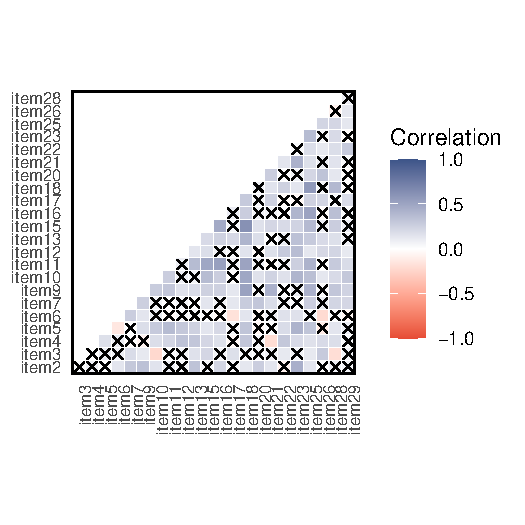
\includegraphics[width=1\linewidth,height=1.5\textheight]{figures/600/corplot} 

}

\caption{Inter-item tetrachoric correlation coefficients for the 23-item Rotter I-E Scale. Inter-item correlation ranged between -.22 to .62. 15.42\% correlations were higher than the absolute value of .30}\label{fig:figCor}
\end{figure}

\begin{table}[tbp]

\begin{center}
\begin{threeparttable}

\caption{\label{tab:map-tab}Minimum Average Partial (MAP) method of factor numder determination. MAP Statistics is the lowest in the 5th row indicating five factors are required.}

\begin{tabular}{llllllll}
\toprule
MAP Statistic & \multicolumn{1}{c}{dof} & \multicolumn{1}{c}{chisq} & \multicolumn{1}{c}{fit} & \multicolumn{1}{c}{RMSEA} & \multicolumn{1}{c}{BIC} & \multicolumn{1}{c}{eChisq} & \multicolumn{1}{c}{SRMR}\\
\midrule
0.01 & 230.00 & 348.16 & 0.32 & 0.04 & -963.71 & 569.29 & 0.06\\
0.01 & 208.00 & 296.79 & 0.37 & 0.04 & -889.59 & 457.10 & 0.05\\
0.01 & 187.00 & 251.80 & 0.42 & 0.03 & -814.81 & 362.14 & 0.05\\
0.01 & 167.00 & 203.85 & 0.46 & 0.03 & -748.68 & 275.86 & 0.04\\
0.02 & 148.00 & 162.38 & 0.51 & 0.02 & -681.78 & 204.50 & 0.04\\
0.02 & 130.00 & 138.05 & 0.54 & 0.01 & -603.44 & 160.76 & 0.03\\
0.02 & 113.00 & 109.60 & 0.57 & 0.00 & -534.92 & 124.69 & 0.03\\
0.03 & 97.00 & 89.70 & 0.60 & 0.00 & -463.56 & 96.41 & 0.03\\
\bottomrule
\end{tabular}

\end{threeparttable}
\end{center}

\end{table}

\begin{lltable}

\begin{longtable}{llllllllllllllllllllllll}\noalign{\getlongtablewidth\global\LTcapwidth=\longtablewidth}
\caption{\label{tab:unnamed-chunk-8}}\\
\toprule
 & \multicolumn{1}{c}{item2} & \multicolumn{1}{c}{item3} & \multicolumn{1}{c}{item4} & \multicolumn{1}{c}{item5} & \multicolumn{1}{c}{item6} & \multicolumn{1}{c}{item7} & \multicolumn{1}{c}{item9} & \multicolumn{1}{c}{item10} & \multicolumn{1}{c}{item11} & \multicolumn{1}{c}{item12} & \multicolumn{1}{c}{item13} & \multicolumn{1}{c}{item15} & \multicolumn{1}{c}{item16} & \multicolumn{1}{c}{item17} & \multicolumn{1}{c}{item18} & \multicolumn{1}{c}{item20} & \multicolumn{1}{c}{item21} & \multicolumn{1}{c}{item22} & \multicolumn{1}{c}{item23} & \multicolumn{1}{c}{item25} & \multicolumn{1}{c}{item26} & \multicolumn{1}{c}{item28} & \multicolumn{1}{c}{item29}\\
\midrule
\endfirsthead
\caption*{\normalfont{Table \ref{tab:unnamed-chunk-8} continued}}\\
\toprule
 & \multicolumn{1}{c}{item2} & \multicolumn{1}{c}{item3} & \multicolumn{1}{c}{item4} & \multicolumn{1}{c}{item5} & \multicolumn{1}{c}{item6} & \multicolumn{1}{c}{item7} & \multicolumn{1}{c}{item9} & \multicolumn{1}{c}{item10} & \multicolumn{1}{c}{item11} & \multicolumn{1}{c}{item12} & \multicolumn{1}{c}{item13} & \multicolumn{1}{c}{item15} & \multicolumn{1}{c}{item16} & \multicolumn{1}{c}{item17} & \multicolumn{1}{c}{item18} & \multicolumn{1}{c}{item20} & \multicolumn{1}{c}{item21} & \multicolumn{1}{c}{item22} & \multicolumn{1}{c}{item23} & \multicolumn{1}{c}{item25} & \multicolumn{1}{c}{item26} & \multicolumn{1}{c}{item28} & \multicolumn{1}{c}{item29}\\
\midrule
\endhead
item2 & 1.00 & 0.04 & 0.09 & 0.01 & 0.14 & 0.30 & 0.34 & 0.15 & 0.09 & 0.05 & 0.33 & 0.06 & 0.23 & 0.03 & 0.13 & 0.27 & 0.14 & -0.08 & 0.44 & 0.14 & 0.00 & 0.09 & 0.07\\
item3 & 0.04 & 1.00 & 0.00 & 0.11 & 0.09 & 0.19 & 0.12 & -0.22 & 0.04 & 0.07 & 0.16 & 0.22 & 0.07 & 0.17 & 0.06 & 0.06 & 0.09 & 0.12 & 0.07 & 0.12 & 0.29 & -0.19 & 0.08\\
item4 & 0.09 & 0.00 & 1.00 & 0.17 & 0.11 & -0.01 & -0.07 & 0.18 & 0.23 & 0.33 & 0.31 & 0.22 & 0.17 & -0.04 & 0.31 & 0.06 & -0.20 & 0.30 & 0.20 & 0.16 & 0.20 & 0.18 & 0.04\\
item5 & 0.01 & 0.11 & 0.17 & 1.00 & -0.14 & 0.00 & 0.18 & 0.29 & 0.37 & 0.30 & 0.25 & 0.14 & 0.21 & 0.05 & 0.32 & -0.05 & 0.01 & 0.19 & 0.42 & 0.32 & -0.11 & 0.14 & 0.09\\
item6 & 0.14 & 0.09 & 0.11 & -0.14 & 1.00 & 0.27 & 0.14 & 0.11 & -0.03 & 0.05 & 0.04 & 0.03 & -0.03 & -0.17 & 0.14 & -0.05 & 0.09 & 0.16 & 0.16 & 0.06 & -0.21 & 0.04 & -0.05\\
item7 & 0.30 & 0.19 & -0.01 & 0.00 & 0.27 & 1.00 & 0.26 & 0.07 & 0.01 & 0.06 & 0.01 & 0.14 & 0.07 & 0.13 & 0.28 & 0.31 & 0.19 & 0.07 & 0.01 & 0.27 & 0.11 & 0.23 & 0.22\\
item9 & 0.34 & 0.12 & -0.07 & 0.18 & 0.14 & 0.26 & 1.00 & 0.28 & 0.31 & 0.16 & 0.19 & 0.25 & 0.25 & 0.13 & 0.52 & 0.04 & 0.43 & 0.02 & 0.11 & 0.43 & 0.03 & 0.31 & 0.24\\
item10 & 0.15 & -0.22 & 0.18 & 0.29 & 0.11 & 0.07 & 0.28 & 1.00 & 0.27 & 0.09 & 0.07 & 0.37 & 0.27 & -0.01 & 0.49 & 0.16 & 0.24 & 0.16 & 0.41 & 0.35 & 0.13 & 0.20 & 0.30\\
item11 & 0.09 & 0.04 & 0.23 & 0.37 & -0.03 & 0.01 & 0.31 & 0.27 & 1.00 & 0.09 & 0.37 & 0.49 & 0.53 & 0.08 & 0.51 & 0.09 & -0.03 & 0.08 & 0.26 & 0.42 & 0.00 & 0.29 & 0.19\\
item12 & 0.05 & 0.07 & 0.33 & 0.30 & 0.05 & 0.06 & 0.16 & 0.09 & 0.09 & 1.00 & 0.14 & 0.18 & 0.07 & 0.05 & 0.15 & -0.03 & 0.17 & 0.29 & 0.36 & 0.13 & 0.21 & 0.23 & 0.12\\
item13 & 0.33 & 0.16 & 0.31 & 0.25 & 0.04 & 0.01 & 0.19 & 0.07 & 0.37 & 0.14 & 1.00 & 0.20 & 0.25 & 0.21 & 0.41 & 0.18 & 0.01 & 0.11 & 0.34 & 0.29 & 0.20 & 0.17 & 0.08\\
item15 & 0.06 & 0.22 & 0.22 & 0.14 & 0.03 & 0.14 & 0.25 & 0.37 & 0.49 & 0.18 & 0.20 & 1.00 & 0.47 & 0.05 & 0.62 & 0.16 & 0.22 & 0.20 & 0.24 & 0.38 & 0.09 & 0.27 & 0.10\\
item16 & 0.23 & 0.07 & 0.17 & 0.21 & -0.03 & 0.07 & 0.25 & 0.27 & 0.53 & 0.07 & 0.25 & 0.47 & 1.00 & 0.10 & 0.27 & 0.08 & 0.07 & 0.01 & 0.41 & 0.51 & -0.02 & 0.35 & 0.04\\
item17 & 0.03 & 0.17 & -0.04 & 0.05 & -0.17 & 0.13 & 0.13 & -0.01 & 0.08 & 0.05 & 0.21 & 0.05 & 0.10 & 1.00 & 0.29 & 0.06 & 0.25 & -0.03 & -0.04 & 0.25 & 0.23 & 0.04 & 0.19\\
item18 & 0.13 & 0.06 & 0.31 & 0.32 & 0.14 & 0.28 & 0.52 & 0.49 & 0.51 & 0.15 & 0.41 & 0.62 & 0.27 & 0.29 & 1.00 & 0.08 & 0.15 & 0.25 & 0.14 & 0.57 & 0.06 & 0.39 & -0.02\\
item20 & 0.27 & 0.06 & 0.06 & -0.05 & -0.05 & 0.31 & 0.04 & 0.16 & 0.09 & -0.03 & 0.18 & 0.16 & 0.08 & 0.06 & 0.08 & 1.00 & 0.27 & 0.02 & 0.08 & 0.22 & 0.33 & 0.13 & -0.02\\
item21 & 0.14 & 0.09 & -0.20 & 0.01 & 0.09 & 0.19 & 0.43 & 0.24 & -0.03 & 0.17 & 0.01 & 0.22 & 0.07 & 0.25 & 0.15 & 0.27 & 1.00 & 0.14 & 0.43 & 0.17 & 0.11 & 0.15 & 0.04\\
item22 & -0.08 & 0.12 & 0.30 & 0.19 & 0.16 & 0.07 & 0.02 & 0.16 & 0.08 & 0.29 & 0.11 & 0.20 & 0.01 & -0.03 & 0.25 & 0.02 & 0.14 & 1.00 & 0.04 & 0.18 & 0.12 & 0.18 & 0.29\\
item23 & 0.44 & 0.07 & 0.20 & 0.42 & 0.16 & 0.01 & 0.11 & 0.41 & 0.26 & 0.36 & 0.34 & 0.24 & 0.41 & -0.04 & 0.14 & 0.08 & 0.43 & 0.04 & 1.00 & 0.37 & 0.05 & 0.20 & -0.02\\
item25 & 0.14 & 0.12 & 0.16 & 0.32 & 0.06 & 0.27 & 0.43 & 0.35 & 0.42 & 0.13 & 0.29 & 0.38 & 0.51 & 0.25 & 0.57 & 0.22 & 0.17 & 0.18 & 0.37 & 1.00 & 0.23 & 0.22 & 0.13\\
item26 & 0.00 & 0.29 & 0.20 & -0.11 & -0.21 & 0.11 & 0.03 & 0.13 & 0.00 & 0.21 & 0.20 & 0.09 & -0.02 & 0.23 & 0.06 & 0.33 & 0.11 & 0.12 & 0.05 & 0.23 & 1.00 & -0.07 & 0.13\\
item28 & 0.09 & -0.19 & 0.18 & 0.14 & 0.04 & 0.23 & 0.31 & 0.20 & 0.29 & 0.23 & 0.17 & 0.27 & 0.35 & 0.04 & 0.39 & 0.13 & 0.15 & 0.18 & 0.20 & 0.22 & -0.07 & 1.00 & 0.10\\
item29 & 0.07 & 0.08 & 0.04 & 0.09 & -0.05 & 0.22 & 0.24 & 0.30 & 0.19 & 0.12 & 0.08 & 0.10 & 0.04 & 0.19 & -0.02 & -0.02 & 0.04 & 0.29 & -0.02 & 0.13 & 0.13 & 0.10 & 1.00\\
\bottomrule
\end{longtable}

\end{lltable}

\begin{figure}

{\centering 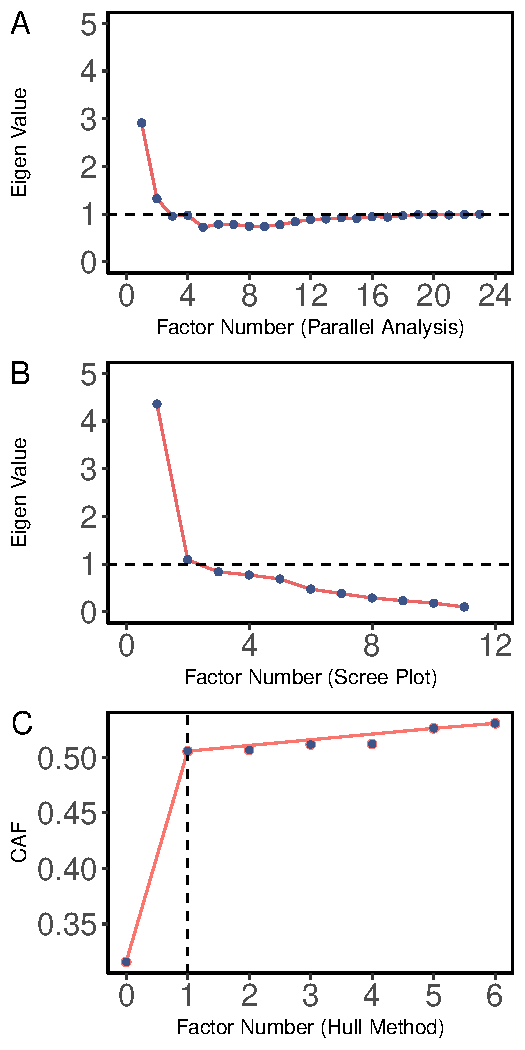
\includegraphics[width=1\linewidth,height=1\textheight]{Figures/600/factors} 

}

\caption{Factor Identification (A) Parallel analysis (B) Scree Plot (C) Hull Method}\label{fig:facIdFig}
\end{figure}

Scree plot ( Fig\ref{fig:facIdFig}) suggested a two-factor solution. In MAP method (Velicer, 1976) the average squared off-diagonal values of the calculated partial correlation matrix are expected to be minimum when the correct number of factors are extracted. In our data set, this value reached the minimum after extracting the first factor. The more contemporary Hull method tries to find an optimal number of factors to balance model fit and the number of parameters (Lorenzo-Seva et al., 2011). This extraction method also supported a 1-factor model. Horn's parallel analysis (Horn, 1965)), like the Monte Carlo study, draws several sets of random data with the same number of participants as the original data set and compares the mean eigenvalues among the simulated and original data sets to retain optimal factors. Parallel analysis is also more immune to the normality assumptions violation(Garrido, Abad, \& Ponsoda, 2013). In our data set parallel analysis with 500 iterations indicated 2 factor solution. As a result, we tested both one factor and two factor solutions.

\begin{table}[tbp]

\begin{center}
\begin{threeparttable}

\caption{\label{tab:TabEFA2}Two Factor Solution}

\begin{tabular}{llllll}
\toprule
item & \multicolumn{1}{c}{WLS1} & \multicolumn{1}{c}{WLS2} & \multicolumn{1}{c}{Communality} & \multicolumn{1}{c}{Uniqueness} & \multicolumn{1}{c}{Complexity}\\
\midrule
item18 & 0.78 &  & 0.667 & 0.333 & 1.175\\
item11 & 0.75 &  & 0.557 & 0.443 & 1.006\\
item15 & 0.65 &  & 0.471 & 0.529 & 1.239\\
item16 & 0.56 &  & 0.324 & 0.676 & 1.051\\
item10 & 0.47 &  & 0.272 & 0.728 & 1.483\\
item5 & 0.45 &  & 0.215 & 0.785 & 1.13\\
item13 & 0.44 &  & 0.216 & 0.784 & 1.235\\
item28 & 0.42 &  & 0.208 & 0.792 & 1.369\\
item4 & 0.38 &  & 0.142 & 0.858 & 1.001\\
item20 &  & 0.64 & 0.409 & 0.591 & 1.013\\
item7 &  & 0.51 & 0.262 & 0.738 & 1.05\\
item21 &  & 0.44 & 0.192 & 0.808 & 1.025\\
item2 &  & 0.37 & 0.162 & 0.838 & 1.334\\
item26 &  & 0.33 & 0.107 & 0.893 & 1.005\\
\% of Variance & 0.2 & 0.1 &  &  & \\
\bottomrule
\end{tabular}

\end{threeparttable}
\end{center}

\end{table}

The initial two-factor solution with all 23 items showed a lack of fit in terms of RMSR value (RMSR =.11), presence of cross-loading items (item9 and item 25) and poor factor loading (\textless.30) items (item6, item22, item29). After discarding these items, we ran another EFA with the remaining 18 items. This iteration of EFA also appeared as a misfit in terms of poor factor loading (Item12). Another five rounds of EFA were conducted with gradually identifying problematic items and discarding them from the model. Finally, a two-factor EFA solution with 14 items was accepted with RMSR = 0.08, no loading smaller than .30 and no cross-loading greater than .30. The first factor retained 9 items, and the second factor retained 5 items. The first factor explained only 20.5\% of the total variance and the second factor explained only 9.6\%. Such low explained variance by the factors were also reported in Marsh and Richards (1987) where they summarized the results of twenty explanatory factor analyses results on Rotter's I-E scale. It was observed that the explained variance by the 1st factor ranged between 7\% to 20\% and the 2nd factor ranges between 7-10\%. The internal consistency of McDonald's omega coefficient for the first factor was satisfactory (Omega = .64). However, the internal consistency of the second factor (Omega = .39) and full scale (Omega = .63) indicated poor internal consistency (Nájera Catalán, 2019).

Next, we fit a one-factor solution, and after 4 rounds of identifying and excluding the problematic items, a simple structure with one factor was obtained with 12 items explaining 32\% of the total variance. The RMSR value was close to the cut-off value (.09). The internal consistency coefficient Mcdonald's omega total was satisfactory (.70).

The obtained one-factor solution retained all items (with additional three items: 4, 9 \& 13) of the first factor obtained in the previous two-factor solution. These items stemmed from the beliefs on the importance of personal ability and effort versus external luck in achieving a desired personal goal. Such a factor in the latent structure of Rotter's I-E scale is supported in the literature (Joe \& Jahn, 1973; Mirels, 1970; Tobacyk, 1978). Our one-factor solution contained all the items retained in the ``personal control'' factor found by Mirels (1970). However the ``political control'' factor (Mirels, 1970; Tobacyk, 1978) reflecting the beliefs on people's influence over political events was not evident in our sample. Items belonging to the second factor of the obtained two-factor model in our study were stemmed from the beliefs on the interpersonal relationship (item7, 20, 26) and misfortune (item21, item 2). This factor was less interpretable and showed low internal consistency (Omega =.39). Thus, we retained the one-factor model, exhibiting better reliability estimates and meaningful interpretation than the two-factor model.

\begin{table}[tbp]

\begin{center}
\begin{threeparttable}

\caption{\label{tab:TabEFA1}}

\begin{tabular}{lll}
\toprule
 & \multicolumn{1}{c}{LOC} & \multicolumn{1}{c}{Communalities}\\
\midrule
item4 & 0.33 & 0.13\\
item5 & 0.45 & 0.18\\
item9 & 0.48 & 0.23\\
item10 & 0.53 & 0.28\\
item11 & 0.69 & 0.48\\
item13 & 0.45 & 0.20\\
item15 & 0.64 & 0.44\\
item16 & 0.61 & 0.39\\
item18 & 0.82 & 0.75\\
item23 & 0.48 & 0.22\\
item25 & 0.69 & 0.51\\
item28 & 0.44 & 0.18\\
\bottomrule
\end{tabular}

\end{threeparttable}
\end{center}

\end{table}

\hypertarget{study-2-confirmation-of-factor-structure-and-psychometric-properties-of-bangla-rotters-i-e-scale}{%
\section{Study 2 Confirmation of Factor Structure and Psychometric Properties of Bangla Rotter's I-E scale}\label{study-2-confirmation-of-factor-structure-and-psychometric-properties-of-bangla-rotters-i-e-scale}}

This study had three objectives. First, to confirm the latent factor structure of Bangla Rotter's I-E scale obtained in the first study by confirmatory factor analysis. Second, to gather validity evidence for our adapted scale (Furr, 2014). Our first study explored the content validity in terms of I-CVI and S-CVI indexes and found satisfactory content validity. Validity evidence for the internal structure would be drawn from the CFA analysis. To check the scale's convergent validity, we calculated the bivariate correlation among the scores of Rotter's I-E scale and Internal Control Index (ICI) (Duttweiler, 1984) and two sub-scales of Big five inventory (O. P. John, Donahue, \& Kentle, 1991) . Third, to gather more information on our adapted scale using the item response theory (IRT)..

\hypertarget{method}{%
\subsection{Method}\label{method}}

\hypertarget{participants-1}{%
\subsubsection{Participants}\label{participants-1}}

A second group of 178 Bangladeshi adults participated in Study 2. They were recruited via email invitation following snowballing techniques. There was no missing or incomplete data. 73\% of the participants was female, ranging in age from 21 to 53 (29.20±4.85) and 27\% of the participants was male, ranging in age from 26 to 44 (33.30±3.82). 78 \% of the participants are married. Average years of education for the males are 16.84±.37 and for the female are 15.14±2.14. For estimating the sample size for the confirmatory factor analysis we followed the N:q rule (Bentler \& Chou, 1987; D. L. Jackson, 2003; Kline, 2015; Worthington \& Whittaker, 2006) where 10 participants per parameters is required to earn trustworthiness of the result. Our sample size exceeds the requirement.

\hypertarget{measures}{%
\subsubsection{Measures}\label{measures}}

\hypertarget{bangla-rotters-i-e-scale}{%
\paragraph{Bangla Rotter's I-E Scale}\label{bangla-rotters-i-e-scale}}

We derived a one-factor solution of the Bangla Rotter's I-E scale by the EFA conducted in our study 1. The internal consistency coefficients for the one-factor model was satisfactory (omega = .70)

\hypertarget{internal-control-index}{%
\paragraph{Internal Control Index}\label{internal-control-index}}

The ICI is a 28-items 5 point scale to measure a person's locus of control (Duttweiler, 1984). The items were translated into Bangla using the standard procedure of forward-backward translation and judgment of an expert panel. Internal consistency coefficient Mcdonald's omega obtained in our sample was .86 indicating satisfactory internal consistency.

\hypertarget{big-five-inventory-bfi}{%
\paragraph{Big Five Inventory (BFI)}\label{big-five-inventory-bfi}}

Previous research has demonstrated the association of Locus of control with different personality factors. External locus of control is associated with high neuroticism (Horner, 1996) and openness to experience (Kobasa et al., 1982; Sherman et al., 1973; Taylor, 1983, 1983) . We decided me measure neuroticism and openness to experience by two sub scales of BFI (Benet-Martínez \& John, 1998; Oliver P. John et al., 2008). We have used the adapted Bangla BFI (Muhammad, Akter, \& Uddin, 2011). The neuroticism sub scale measures the extent to which an indivudual is affectively unstable, anxious and worried(Horner, 1996).It has 8 items (3 reversed items). The openness subscale has 10 items (2 reversed items) and measures individual's susceptibility to aesthetics, ideas, values and flexibility(Costa \& McCrae, 1992). Each item (except for the reversed items) was scored on a five point Likert scale ranging from 1 (completely disagree) to 5 (completely agree) Test-retest reliabilities of the Bengali version of BFI for neuroticism {[}r =.92, p \textless{} 0.01{]} and openness {[}r = .87, p \textless{} 0.01{]} was satisfactory (Muhammad et al., 2011).

\hypertarget{procedure-1}{%
\subsubsection{Procedure}\label{procedure-1}}

Participants were invited to participate voluntarily in the online study. Once agreed, participants' consent was digitally recorded, and data collection commenced.

\hypertarget{results-and-discussion}{%
\subsubsection{Results and Discussion}\label{results-and-discussion}}

We used the `Lavaan'(Rosseel, 2012) package in Rstudio to conduct the categorical confirmatory factor analysis with robust weighted least square (WLSMV) estimator as our response data was dichotomous (Brown, 2015). Commonly used Model fit benchmarks of Hu and Bentler (1999) focused on (i) the comparative fit index (CFI;) (ii) the Tucker Lewis index (TLI) (CFI/TLI, \(goodfit \geq .95\), \(acceptable fit\geq .90\)) (ii) the root mean square error of approximation (RMSEA; close to .06 or below), (iii) the standardized root mean square (SRMR; close to .08 or below) to estimate the model fit. Additionally, the chi-square test is also used to estimate the absolute model fit. Table \ref{tab:tabCfa} summarizes the fit indices of our fitted model. The fitted model failed to attain an absolute fit estimated by the chi-square test. It is necessary to keep in mind that the chi-square test is sensitive to sample size while estimating the model and not recommended to be used as the sole index of absolute model fit (Brown, 2015). SRMR value was also higher than general guideline. It is evident from the work of ({[}Generic{]}, 2002) that for categorical data SRMR performs poorly. Subsequently we judged the model fit based on incremental and parsimony fit indices values. Incremental fit indices for the one factor model (CFI =.92, TLI = .91) and parsimony index (RMSEA = .04) were indicating acceptable fit. However, one item (item23) loaded poorly. By discarding the item one factor model attained best fit (CFI =.98, TLI = .97, RMSEA = .00). SRMR value (.10) was also close to the suggested guideline(.08) The internal consistency reliability coefficients McDonald's omega value for both models were satisfactory (.71 \& .72, respectively). Fig\ref{fig:figcfa} depicts both model.

\begin{table}[tbp]

\begin{center}
\begin{threeparttable}

\caption{\label{tab:tabCfa}Fit Indices Of CFA}

\begin{tabular}{llllllll}
\toprule
Model & \multicolumn{1}{c}{Chi-Squre} & \multicolumn{1}{c}{df} & \multicolumn{1}{c}{CFI} & \multicolumn{1}{c}{TLI} & \multicolumn{1}{c}{RMSEA} & \multicolumn{1}{c}{SRMR} & \multicolumn{1}{c}{McDonald's Omega}\\
\midrule
One Factor Model & 83.84 & 54 & .92 & .91 & .04 & .13 & .72\\
One Factor Model Modified & 72.24 & 53 & .98 & .97 & .00 & .10 & .72\\
\bottomrule
\end{tabular}

\end{threeparttable}
\end{center}

\end{table}

\begin{figure}
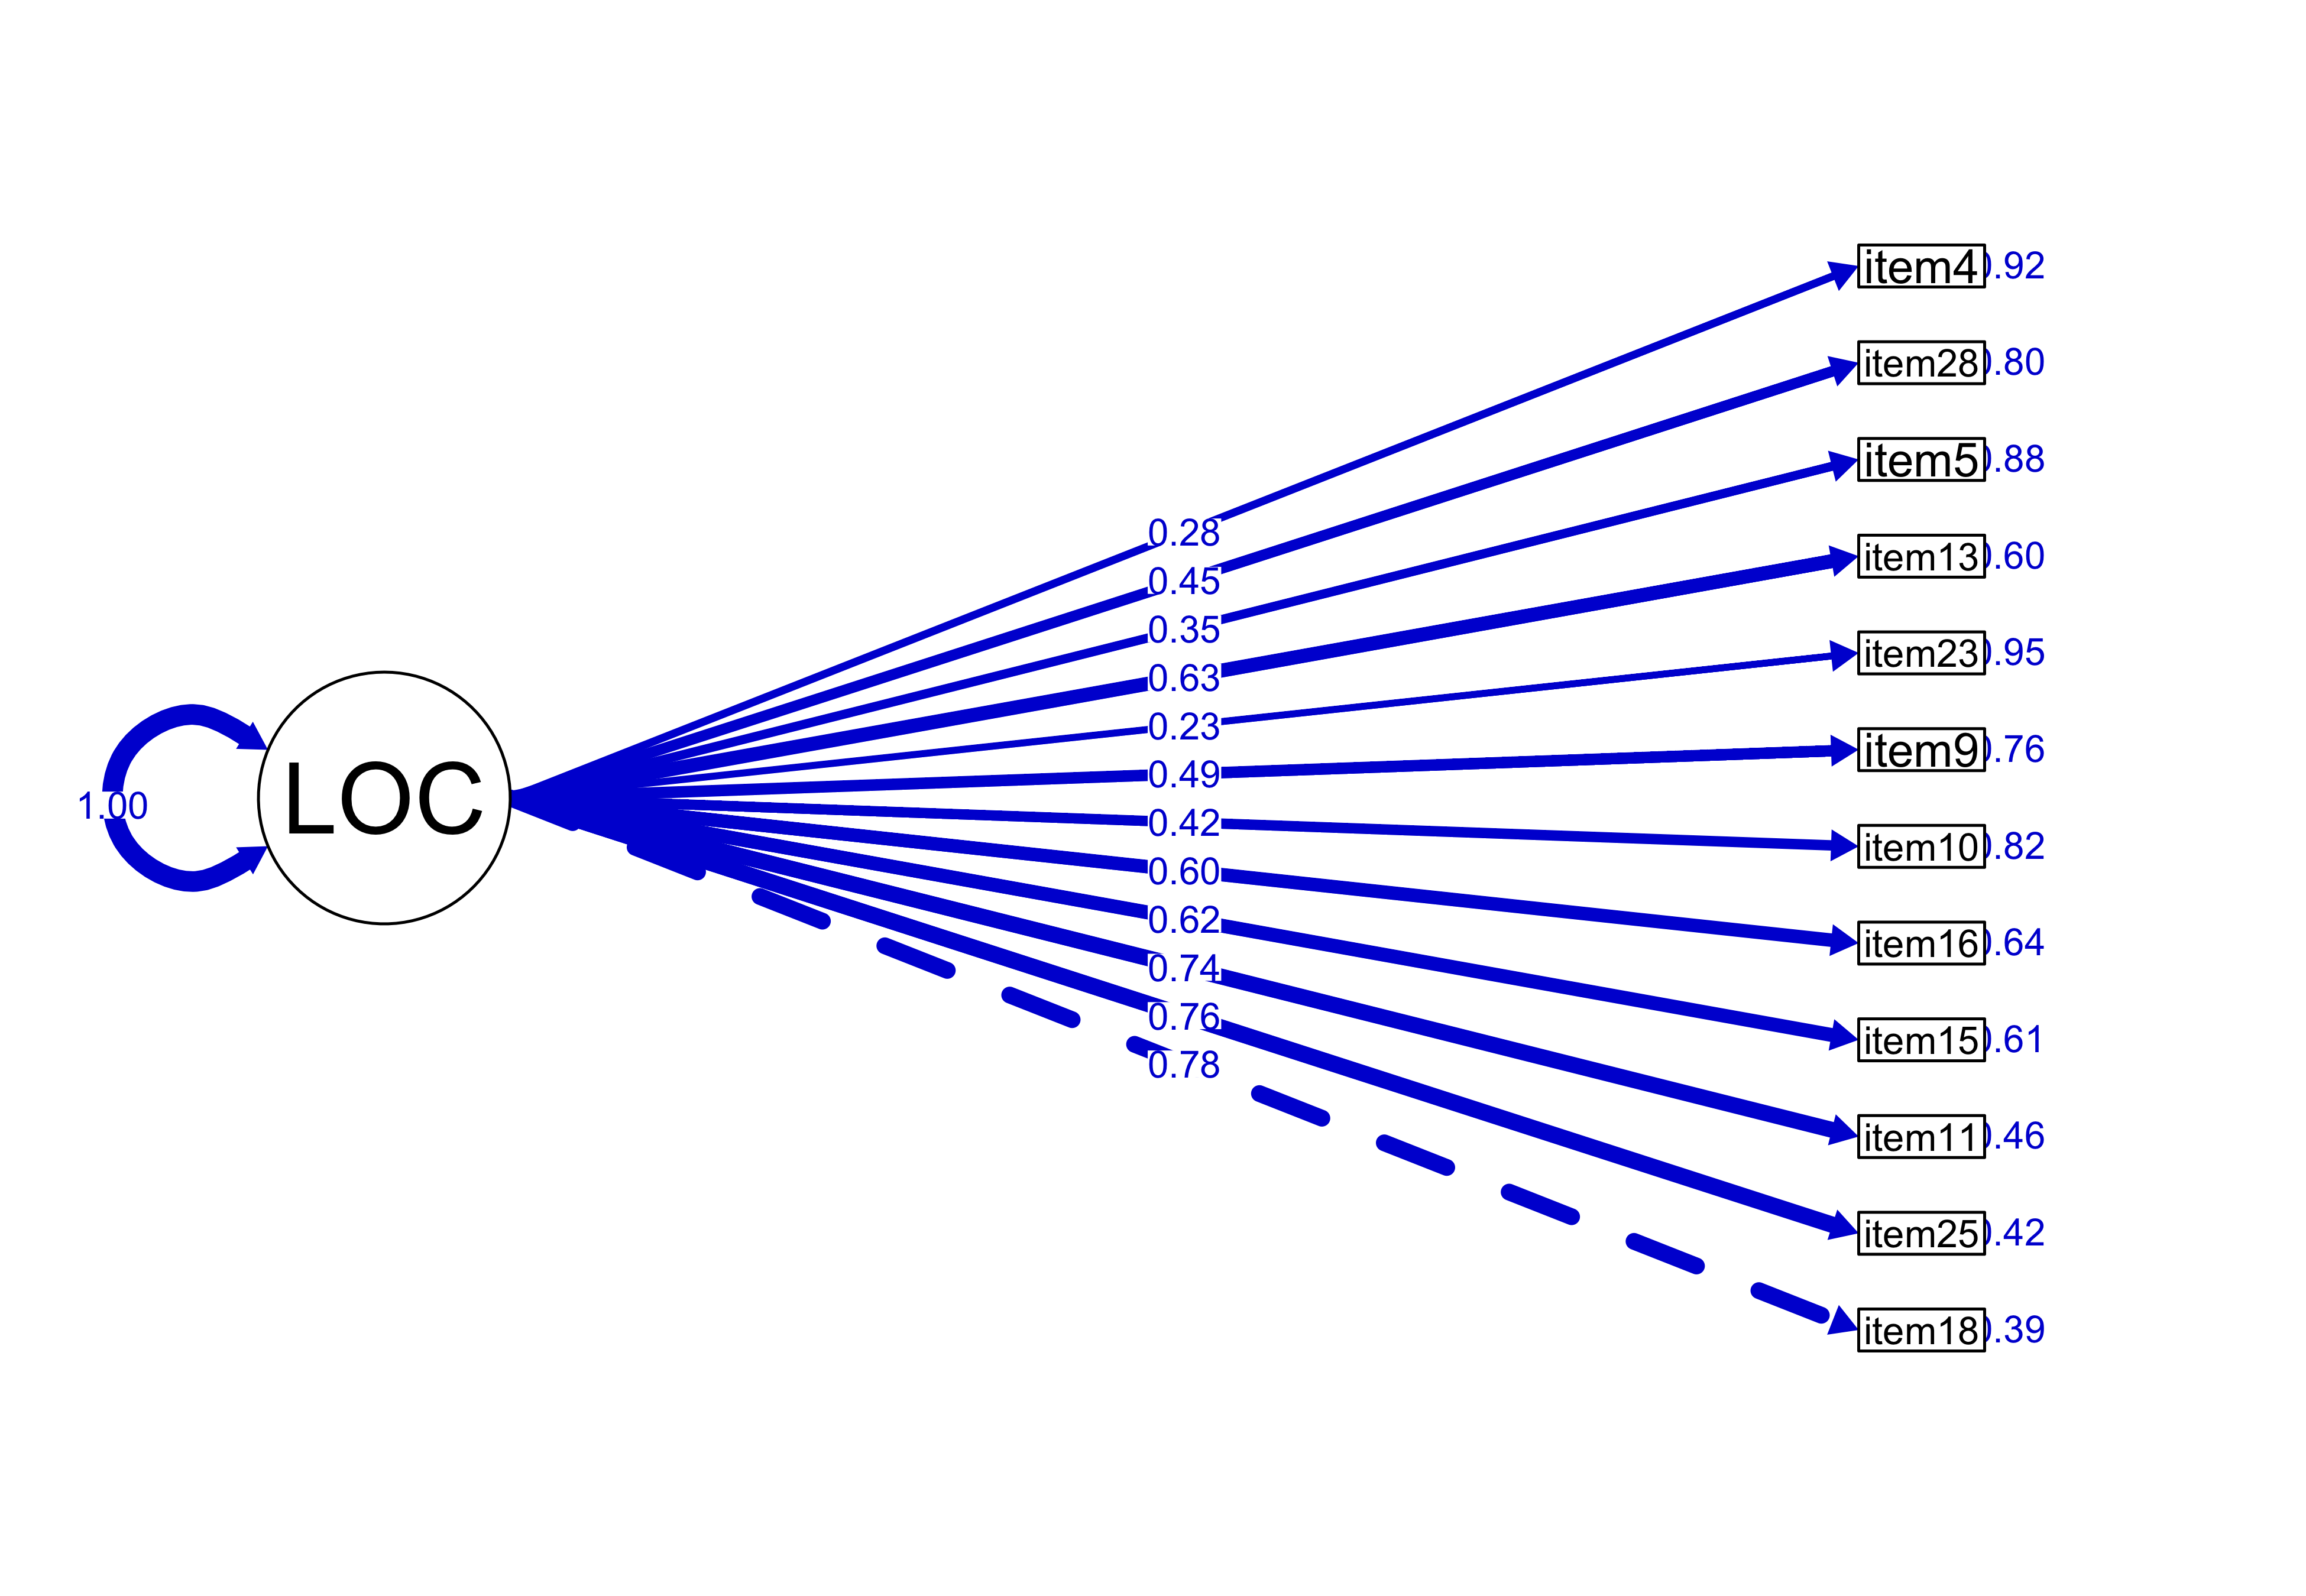
\includegraphics[width=0.5\linewidth]{Rotterpaper_files/figure-latex/figcfa-1} 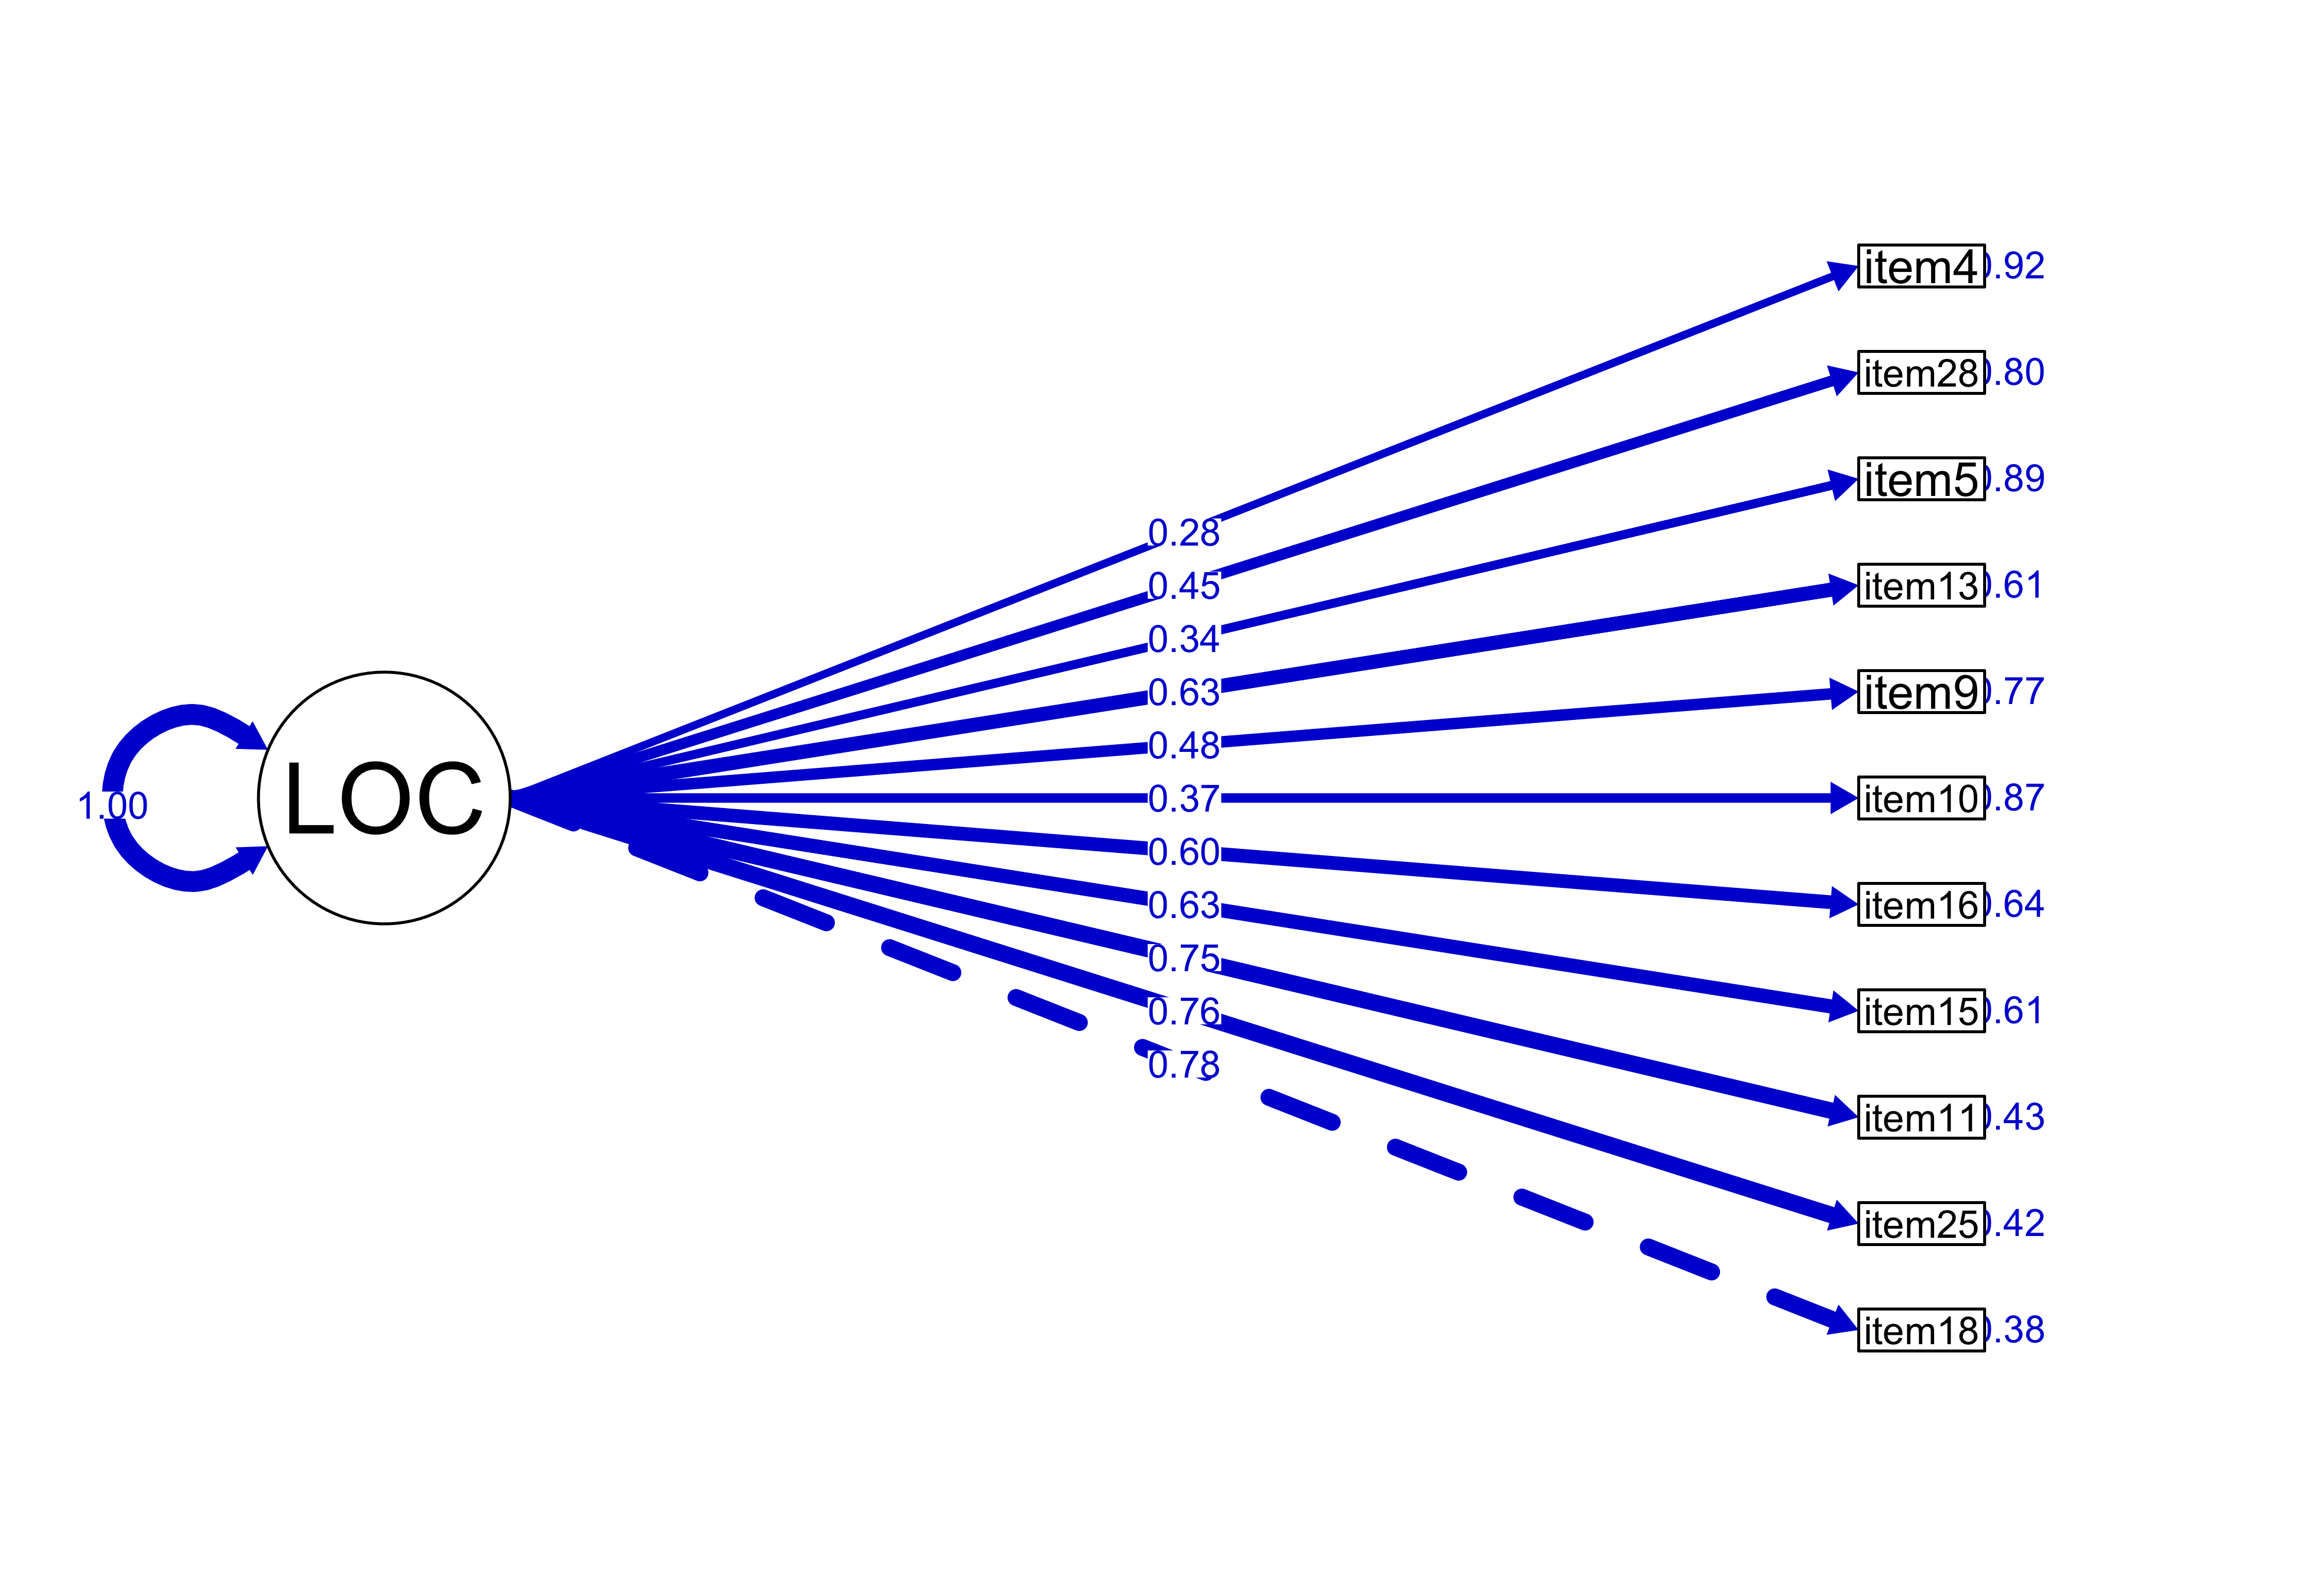
\includegraphics[width=0.5\linewidth]{Rotterpaper_files/figure-latex/figcfa-2} \caption{(A) One Factor Model of Bangla Rotter's I-E Scale (12 Items), (B) One Factor Model (11 Items)}\label{fig:figcfa}
\end{figure}

\hypertarget{the-validity-of-bangla-rotters-i-e-scale}{%
\subsubsection{The Validity of Bangla Rotter's I-E Scale}\label{the-validity-of-bangla-rotters-i-e-scale}}

We have gathered satisfactory content validity evidence of Rotter's I-E scale in our first study by I-CVI and S-CVI. Our second study gathered structural validity evidence by confirming the one-factor solution obtained in the EFA. Lastly, we gathered convergent validity evidence based on correlational analysis among the total score of ICI (Duttweiler, 1984), neuroticism, openness to experience (Muhammad et al., 2011) and Bangla Rotter's I-E scale

Table\ref{tab:tabvalidity} summarized the correlation coefficients. Bangla Rotter's I-E scale were significantly positively correlated with neuroticism, r = .21, p\textless0.01. Such a significant positive correlation was also reported in Horner (1996), r = 0.33, p\textless.001. Internal control index (ICI) showed a significant negative correlation, r = -.22, p\textless.01. Duttweiler (1984) also reported such correlation, r = -.39, p\textless.01 between the ICI and ``personal control'' factor of Mirels (1970). Openness to experience also showed a significant negative correlation with Bangla Rotter's I-E scale, r = -.22, p \textless.001. Rodrigues and Deuskar (2018) also reported such significant negative correlation of between LoC and openness to experience (r= -.22, p \textless0.01)

\hypertarget{irt-analysis}{%
\subsubsection{IRT Analysis}\label{irt-analysis}}

To gather more information on our retained one-factor solution, we sought Item Response Theory (IRT). IRT complements the conventional classical test theory-based analysis by gathering information on item discrimination and item difficulty. IRT judges an item's quality by providing item information in the light of participants' trait level (\(\theta\)). We gathered evidence on item quality as well as item fit, person fit and model by fitting a two-parameter logistic model (2PL) model to the combined EFA sample and CFA sample (n =532) in RStudio with the ``mirt'' package (Chalmers, 2012). We did a Monte Carlo simulation using ``SimDesign'' package (Chalmers \& Adkins, 2020) with sample sizes varying from 50-350 and calculated average root mean squared error(RMSE) to estimate the optimal sample size for the 2PL model with 11 items. The RMSE became stable for n = 200 to 300 (RMSE ranging between .25-.32). Our combined sample size was larger than the estimated sample size for stability.

It required 16 iterations (Log-likelihood -3152.126) for the 2PL model to converge. Item fit statistics signed chi-square test (S-X2)(Orlando \& Thissen, 2000, 2003) indicated all items were a good fit. Model fit statistics estimated from the model indicated a best fit for the the 2PL model, M2 = 59.42, df = 44, p= .06, RMSEA = .03{[}.00 - .04{]}, CFI = .98, TLI = .98.

\begin{figure}
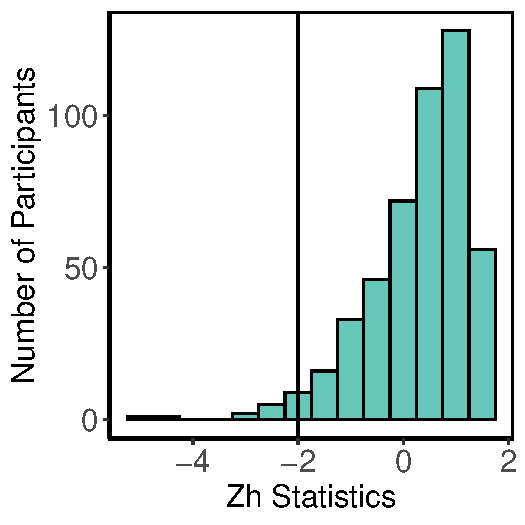
\includegraphics[width=3.5in]{Figures/600/personfit} \caption{Distribution of the Zh statistic of 2PL model}\label{fig:figfmisfit}
\end{figure}

Person fit indicates the validity and meaningfulness of the fitted model at the participants latent trait level (Embretson \& Reise, 2000). We estimated the person fit statistics using standardized fit index Zh statistics (Drasgow, Levine, \& Williams, 1985). Zh \textless{} -2 should be considered as a misfit. Fig\ref{fig:figfmisfit} indicates that Zh is larger than -2 for most participants, suggesting a good fit of the selected IRT model.

\begin{table}[tbp]

\begin{center}
\begin{threeparttable}

\caption{\label{tab:tabIRT}IRT Description}

\begin{tabular}{llllllll}
\toprule
Items & \multicolumn{1}{c}{Discrimination} & \multicolumn{1}{c}{Difficulty} & \multicolumn{1}{c}{S-X2} & \multicolumn{1}{c}{df} & \multicolumn{1}{c}{p} & \multicolumn{1}{c}{outfit} & \multicolumn{1}{c}{infit}\\
\midrule
item18 & 2.21 & -1.09 & 6.42 & 4.00 & .17 & 0.65 & 0.75\\
item25 & 1.64 & -0.55 & 9.82 & 6.00 & .13 & 0.73 & 0.82\\
item11 & 1.80 & -0.04 & 2.96 & 6.00 & .81 & 0.65 & 0.77\\
item15 & 1.41 & -0.14 & 3.78 & 6.00 & .71 & 0.77 & 0.84\\
item16 & 1.47 & 0.78 & 2.52 & 6.00 & .87 & 0.75 & 0.83\\
item10 & 0.96 & 2.79 & 9.33 & 6.00 & .16 & 0.80 & 1.02\\
item9 & 0.95 & 0.98 & 4.24 & 7.00 & .75 & 0.86 & 0.93\\
item13 & 0.98 & -0.16 & 5.21 & 7.00 & .63 & 0.88 & 0.91\\
item5 & 0.77 & 2.40 & 4.41 & 7.00 & .73 & 0.92 & 0.98\\
item28 & 0.87 & 1.55 & 1.04 & 7.00 & .99 & 0.89 & 0.95\\
item4 & 0.49 & 0.31 & 9.94 & 7.00 & .19 & 0.97 & 0.97\\
\bottomrule
\end{tabular}

\end{threeparttable}
\end{center}

\end{table}

We categorize the item discrimination in table\ref{tab:tabIRT} using the following criteria of F. B. Baker (2017), none = 0; very low =0.01 to 0.34; low = 0.35 to 0.64; moderate = 0.65 to 1.34 ; high = 1.35 to 1.69; very high \textgreater1.70. Among the 11 items, 6 items showed moderate discrimination and one item showed high discrimination (item16). Three items (item 18, 25 \& 11) had very high discrimination and one item (item 4) had low discrimination. All items were in the suggested guidelines of item discrimination parameter: 0.5\(\le\) Item Discrimination \(\le\) 2.0 (except items 18 \& 4), and the item difficulty parameters: -3.0 \(\le\) Item Difficult\(\le\) 3.0 (F. B. Baker, 2017). The relationship between participants' latent traits and the probability of responding to the preferred response option for the items is shown by the item characteristics curve (ICC) (Figure\ref{fig:IIC}). For an easy item to have a probability of .50 a latent trait level \(\theta\) = -1 is required for easy items, \(\theta\) = 0 is required for moderate items and \(\theta\) = 1 is required for hard items (Desjardins \& Bulut, 2018). Examination of the ICCs made it evident that our adapted scale contained all three types of items with item difficulty parameters ranging from -1.06 to 2.88, reflecting a sizable range of underlying locus of control trait.

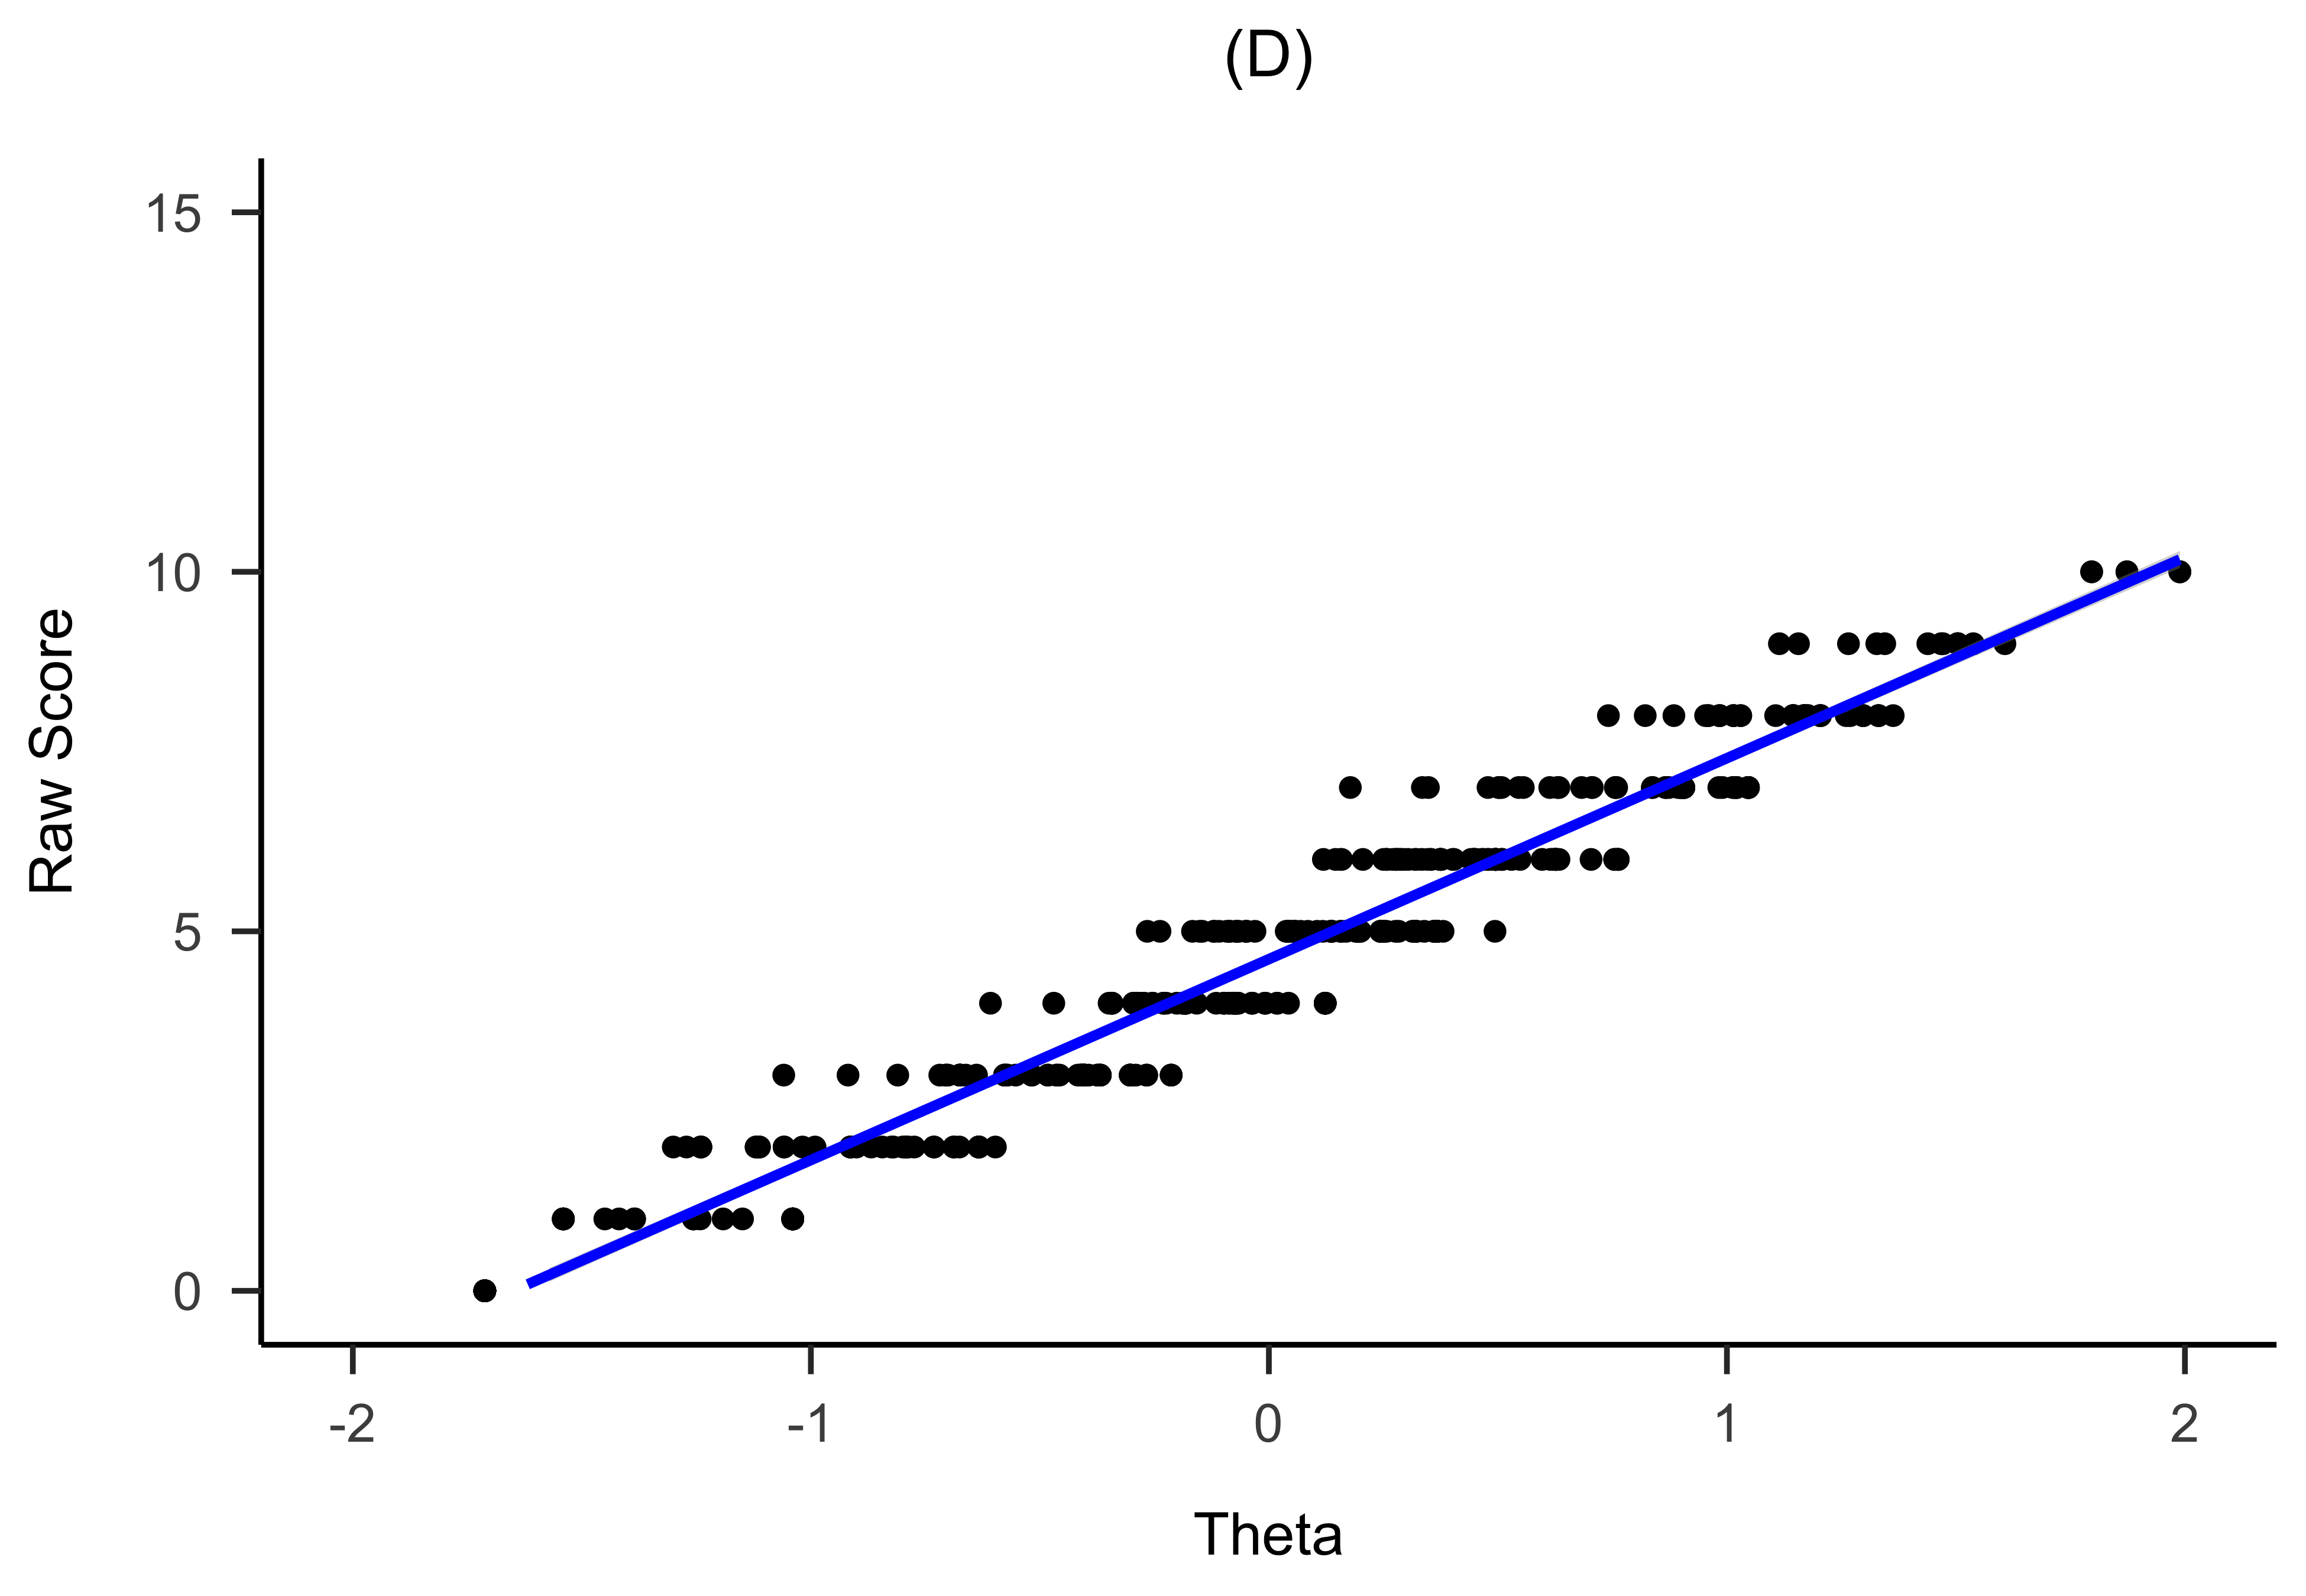
\includegraphics{Rotterpaper_files/figure-latex/irt-plots-1.png}

Item information curve (IIC) and test information curve (TIC) indicate the amount of information an item and the full scale carry along the latent trait continuum, respectively (Figure\ref{fig:IIC}). Examination of the IICs' revealed that item 18 carried the highest information between \(\theta\) level -2 to 1. Item 4 was not very informative with almost flat IIC along the trait. Item 11, 13, 15, and 25 have a little information bump centered on the measured trait (\(\theta\)). Item 5, 9, 10, 16 and 28 have a little bump of information located on the external locus of the control area. Test information curve (\ref{fig:figTIC}. also indicated the test had the least measurement error between \(\theta\) = -1 and \(\theta\) = 0. The amount of information changed rather steadily with the change of \(\theta\) across the continuum. Thus we conferred the ability was estimated with precision near the center of the locus of control scale (F. B. Baker, 2017) with a peak in the ranges of \(\theta\) = -1 and \(\theta\) = 0, which is sufficient to discriminate between external locus of control and internal locus of control. This Adequacy is reflected by the correlation coefficient of the estimated \(\theta\) and the obtained score in the Rotter's I-E scale, r =.98, p \textless{} .01 (\ref{fig:figICC}.

\begin{figure}
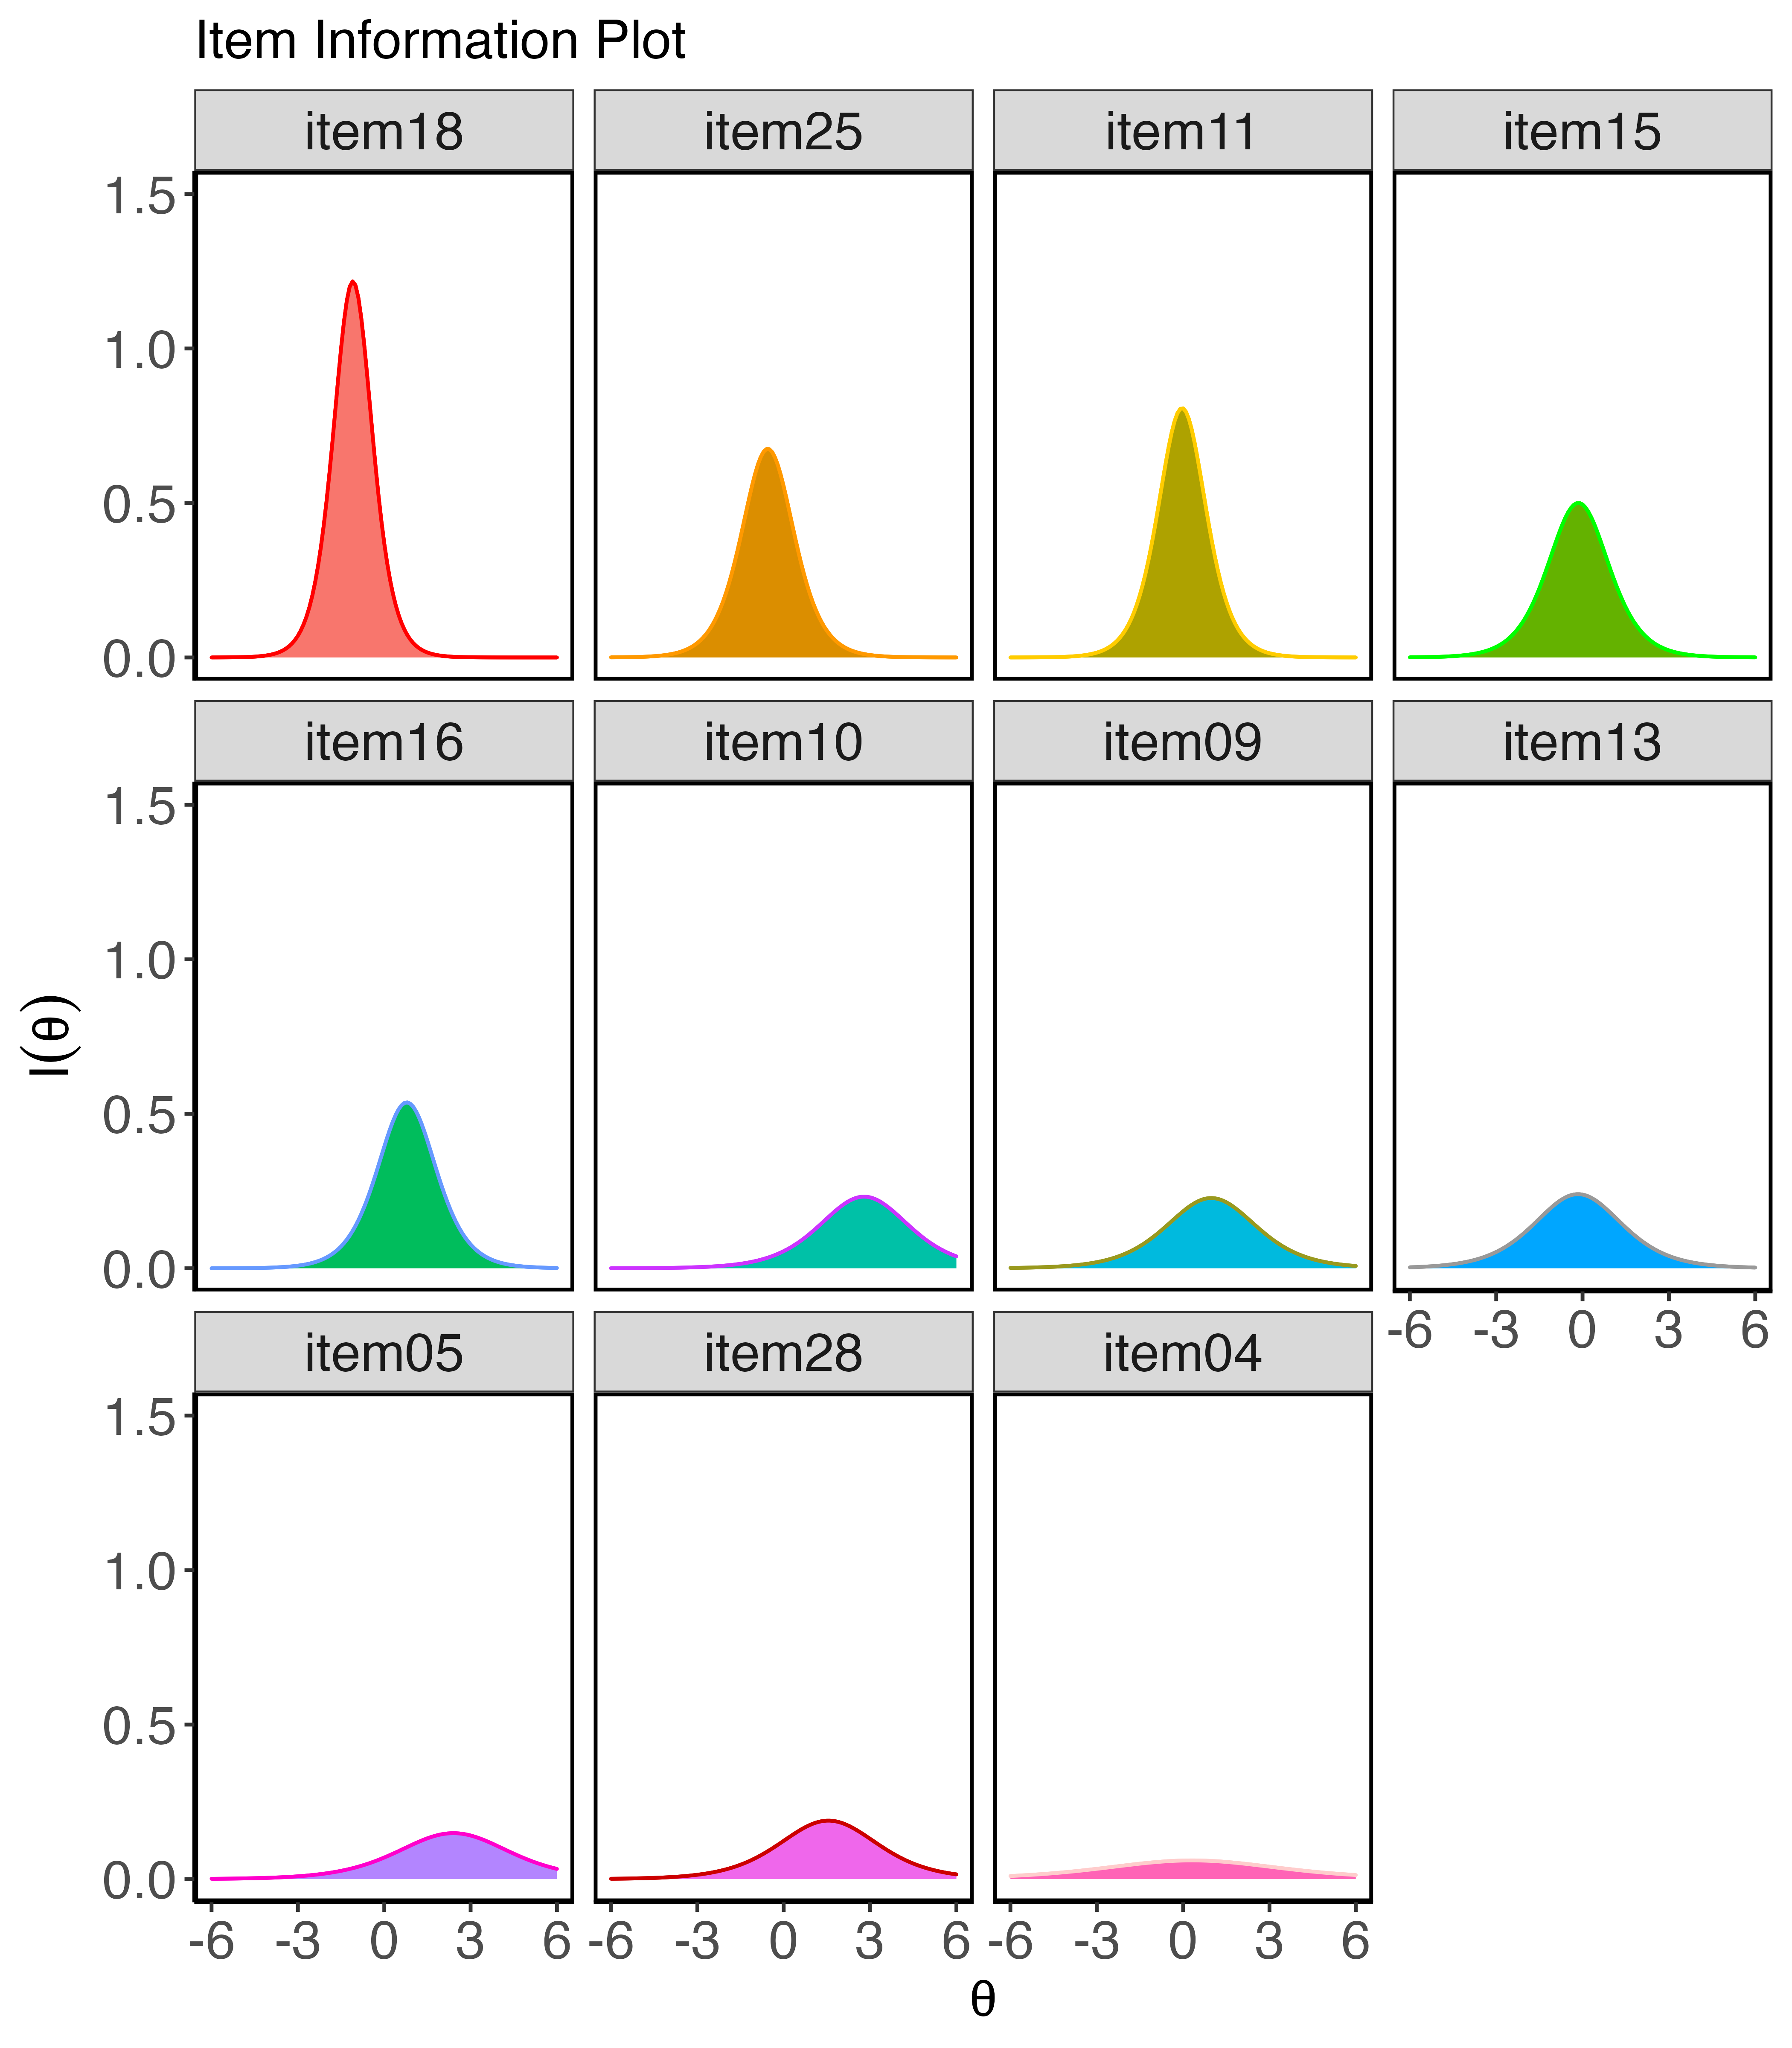
\includegraphics[width=7in]{Figures/600/ifc} \caption{Item Information Curves of Bangla Rotter’s I-E Scale. Item 18 carried the highest level of information across the theta continuum and item 04 carried the lowest information}\label{fig:FigTIC}
\end{figure}

\begin{figure}
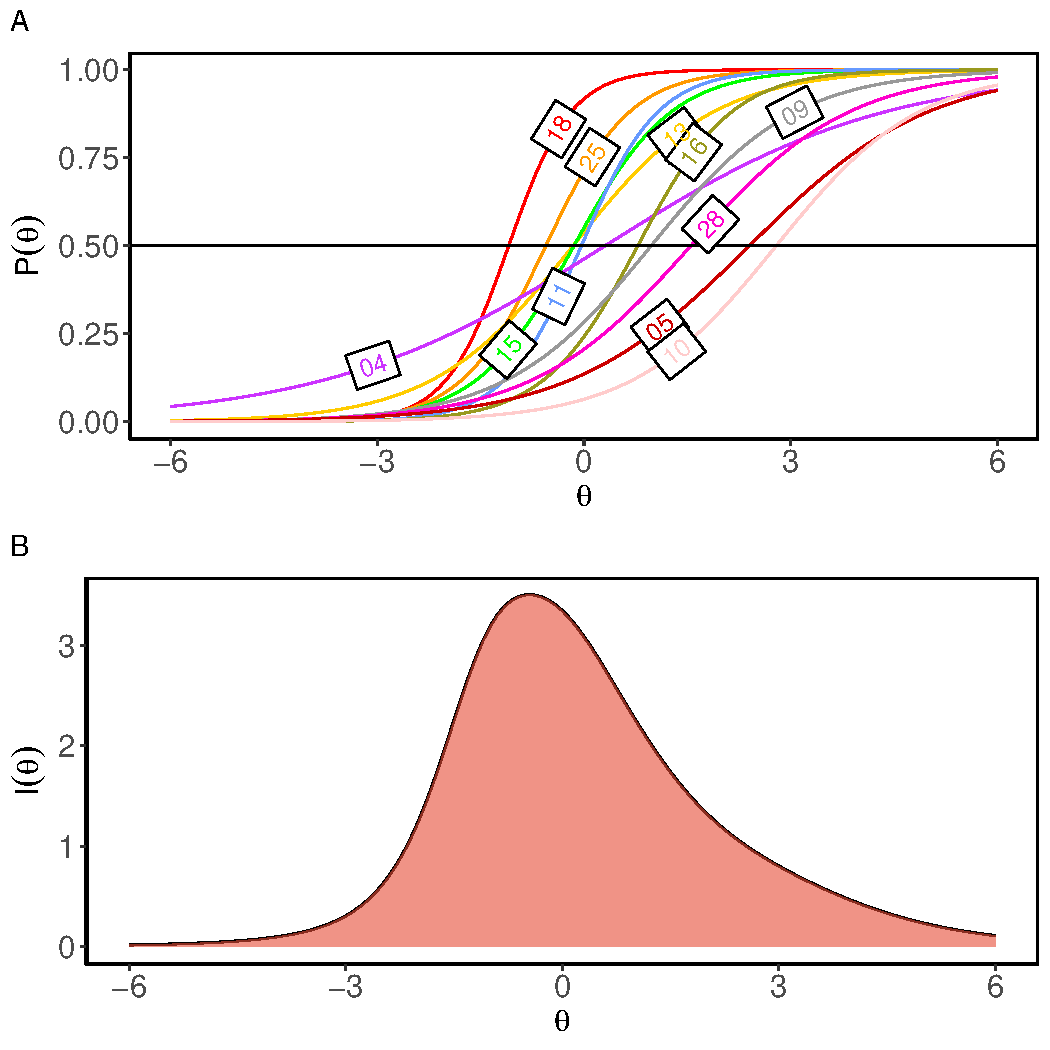
\includegraphics[width=7in]{Figures/600/icc_tic} \caption{(A) Item Characteristic Curves (ICC) of the 11 items of the Bangla Rotter I-E scale. ICC indicates Bangla Rotter I-E scale is composed of items with easy, moderate and hard items. (B) Test information Curve. The peak of the curve centered near the center of the continuum between the theta range -1 to 0.}\label{fig:figICC}
\end{figure}

\hypertarget{general-discussion}{%
\section{General Discussion}\label{general-discussion}}

We followed the ICT (Bartram et al., 2018) guidelines to culturally adapt the Rotter's I-E scale and psychometrically evaluate it by gathering evidence of validity (content, structural, and convergent)(Furr, 2014) and estimating reliability (Internal consistency). We also gathered information about item quality using item response theory.

We confirmed the construct equivalence of locus of control in both the western and eastern cultures by a robust literature review. Then we started with the initial 23 (except the six filler items) original items and translated them into Bangla following the standard forward-backward translation procedure (Study 1). The content validity of the initial synthesized scale was assessed by I-CVI and S-CVI (average) (Lynn, 1986; Polit et al., 2007) from the evaluation of 8 mental health experts. The final I-CVI scores for each item were higher than 0.83 and S-CVI was .94 indicating satisfactory content validity (Lynn, 1986; Polit et al., 2007). We administered the scale to a large sample (300) of elementary school teachers to explore the latent construct structure. In exploratory factor analysis, we obtain two solutions: a one-factor solution with 12 items and a two-factor solution with 14 items. However, only the one-factor solution and the first factor of the two-factor solution yielded acceptable internal consistency (McDonald's omega .70 \&.64 respectively)(Nájera Catalán, 2019). Both of these factors contained similar items stemming from the beliefs regarding personal control over desired goal attainment. The emergence of such a factor is in line with the previous research (Mirels, 1970; Tobacyk, 1978). This emerged factor described the respondent's preference to assign greater or lesser value to personal ability than to luck in realizing the desired goal. Each of these items posed statements (e.g., In the long run, people get the respect they deserve in this world/Unfortunately, an individual's worth often passes unrecognized no matter how hard he tries) which would affirm the respondents' disposition on their fate vs.~to their ability and hard work. The second factor of the two-factor solution contained 5 items stemming from beliefs on interpersonal relationships and control over misfortune. However, this factor was less interpretable in terms of a common theme and showed a poor reliability estimate ( McDonald's Omega =.39). As a result, we accepted the one-factor solution.

A CFA on a separate sample (Study 2) indicated the best fit of one-factor solution (CFI =.97, TLI = .96, RMSEA = .04).The internal consistency of the scale measured by McDonald's omega was also above the suggested criteria for both EFA and CFA samples (McDonald's Omega =.70). We gathered validity evidence by estimating correlations between our scale and neuroticism, openness to experience (Muhammad et al., 2011) and internal control index (Duttweiler, 1984). The ICI (Duttweiler, 1984) measures the same construct, LoC, and a high score would indicate the internal locus of control. On our scale, a high score would indicate an external locus of control. Thus a negative correlation is expected. Our scale showed a significant negative yet low correlation (r = -.21, p\textless.01). Duttweiler (1984) also reported moderate negative correlation between ICI and and Mirels' (1970) ``personal control' factor. They attributed the cause of such moderate correlation to the limited focus of the items in the''personal control' factor. Like Mirels'(1970), items retained in our scale limit their focus to the person's disposition on luck or personal ability to attain the desired goal. Whereas ICI encompasses items that also focus on self-image, and willingness to take action. As a result, such a correlation is expected.

Locus of control is believed to be correlated with behaviors and emotions related to neuroticism such as maladaptive coping strategies (Taylor, 1983) and depression (Benassi, Sweeney, \& Dufour, 1988). Previous studies reported external locus of control positively correlate to neuroticism (Horner, 1996; Morelli, Krotinger, \& Moore, 1979). Bangla Rotter's I-E scale also showed significant positive correlation with neuroticism, (r = .22, p \textless0.01). Literature also suggests the externals would score low on openness to experinece personality trait (Rodrigues \& Deuskar, 2018; Sherman et al., 1973). Bangla Rotter's I-E scale showed a significant negative correlation with openness to experience , r = -.22, p\textless.001. From these gathered evidence of validity we conferred our adapted scale has satisfactory convergent validity.

Lastly, we gathered more information on the item quality of the retained items in our scale by Item response theory. We fitted a two-parameter logistic model (2PL) (Thissen, 2015) to our data. The fit indices indicated a best fit of the model, (M2 = 59.42, df = 44, p= .06, RMSEA = .03{[}.00 - .04{]}, CFI = .98, TLI = .98). Only one item was identified as a misfit item (item4). However, our IRT analysis aimed to gather as much information as possible on the items, not to discard any. As such, we retained all the items obtained in our one-factor solution. In terms of item difficulty, our scale contained items of all categories: easy, moderate and hard items and covered a substantial range of underlying locus of control attributes. Additionally, all items except item18 were also exhibiting item discrimination within the suggested range (F. B. Baker, 2017). Test information curve also indicated adequate ability to discriminate between external locus of control and internal locus of control with precision as the peak of the curve centered near the center of the continuum at \(\theta\) = -1 and \(\theta\) = 0. Also, the high correlation of estimated \(\theta\) score and the obtained score ( r =.98 , p\(\le\).01) in our scale indicated the adequacy of our adapted scale.

Based on the psychometric analysis conducted, we recommend that researchers use this scale to measure an individual's locus of control with precision. The scale can potentially be used in clinical and counseling settings to identify the LoC, thus facilitating the therapeutic process.

\hypertarget{future-directions}{%
\section{Future Directions}\label{future-directions}}

We recommend some works for future researchers. First, geographically the scope of the data was narrow; data from other parts of the country should be considered to widen the scope. Second, the differential item functioning and measurement invariance can be analyzed for males and females and age groups to identify potential item bias.

\newpage

\hypertarget{references}{%
\section{References}\label{references}}

\begingroup
\setlength{\parindent}{-0.5in}
\setlength{\leftskip}{0.5in}

\hypertarget{refs}{}
\begin{CSLReferences}{1}{0}
\leavevmode\vadjust pre{\hypertarget{ref-R-equate}{}}%
Albano, A. D. (2016). {equate}: An {R} package for observed-score linking and equating. \emph{Journal of Statistical Software}, \emph{74}(8), 1--36. \url{https://doi.org/10.18637/jss.v074.i08}

\leavevmode\vadjust pre{\hypertarget{ref-andriessen1983analysis}{}}%
Andriessen, J., \& Van Cadsand, J. (1983). An analysis of the dutch IE scale. \emph{Nederlands Tijdschrift Voor de Psychologic}, \emph{38}, 7--24.

\leavevmode\vadjust pre{\hypertarget{ref-R-papaja}{}}%
Aust, F., \& Barth, M. (2020). \emph{{papaja}: {Prepare} reproducible {APA} journal articles with {R Markdown}}. Retrieved from \url{https://github.com/crsh/papaja}

\leavevmode\vadjust pre{\hypertarget{ref-baker1979relationship}{}}%
Baker, E. K. (1979). The relationship between locus of control and psychotherapy: A review of the literature. \emph{Psychotherapy: Theory, Research \& Practice}, \emph{16}(3), 351.

\leavevmode\vadjust pre{\hypertarget{ref-RN1275}{}}%
Baker, F. B. (2017). \emph{The basics of item response theory using r} (1st ed. 2017.). Springer.

\leavevmode\vadjust pre{\hypertarget{ref-RN1233}{}}%
Bandalos, D. L., \& Finney, S. J. (2018). Factor analysis: Exploratory and confirmatory. In \emph{The reviewer's guide to quantitative methods in the social sciences} (pp. 98--122). Routledge.

\leavevmode\vadjust pre{\hypertarget{ref-bandura1977social}{}}%
Bandura, A., \& Walters, R. H. (1977). \emph{Social learning theory} (Vol. 1). Englewood cliffs Prentice Hall.

\leavevmode\vadjust pre{\hypertarget{ref-R-questionr}{}}%
Barnier, J., Briatte, F., \& Larmarange, J. (2021). \emph{Questionr: Functions to make surveys processing easier}. Retrieved from \url{https://CRAN.R-project.org/package=questionr}

\leavevmode\vadjust pre{\hypertarget{ref-R-tinylabels}{}}%
Barth, M. (2021). \emph{{tinylabels}: Lightweight variable labels}. Retrieved from \url{https://github.com/mariusbarth/tinylabels}

\leavevmode\vadjust pre{\hypertarget{ref-RN1261}{}}%
Bartlett, M. (1954). A note on the multiplying factors for various chi-square approximations. \emph{Journal of the Royal Statistical Society. Series B, Methodological}, \emph{16}(2), 296--298.

\leavevmode\vadjust pre{\hypertarget{ref-RN1156}{}}%
Bartram, D., Berberoglu, G., Grégoire, J., Hambleton, R., Muniz, J., \& Vijver, F. van de. (2018). ITC guidelines for translating and adapting tests (second edition). \emph{International Journal of Testing}, \emph{18}(2), 101--134. \url{https://doi.org/10.1080/15305058.2017.1398166}

\leavevmode\vadjust pre{\hypertarget{ref-R-lme4}{}}%
Bates, D., Mächler, M., Bolker, B., \& Walker, S. (2015). Fitting linear mixed-effects models using {lme4}. \emph{Journal of Statistical Software}, \emph{67}(1), 1--48. \url{https://doi.org/10.18637/jss.v067.i01}

\leavevmode\vadjust pre{\hypertarget{ref-R-Matrix}{}}%
Bates, D., \& Maechler, M. (2021). \emph{Matrix: Sparse and dense matrix classes and methods}. Retrieved from \url{https://CRAN.R-project.org/package=Matrix}

\leavevmode\vadjust pre{\hypertarget{ref-benassi1988}{}}%
Benassi, V. A., Sweeney, P. D., \& Dufour, C. L. (1988). Is there a relation between locus of control orientation and depression? \emph{Journal of Abnormal Psychology}, \emph{97}(3), 357.

\leavevmode\vadjust pre{\hypertarget{ref-RN1279}{}}%
Benet-Martínez, V., \& John, O. P. (1998). Los cinco grandes across cultures and ethnic groups: Multitrait multimethod analyses of the big five in spanish and english. \emph{Journal of Personality and Social Psychology}, \emph{75}(3), 729--750. \url{https://doi.org/10.1037/0022-3514.75.3.729}

\leavevmode\vadjust pre{\hypertarget{ref-R-effectsize}{}}%
Ben-Shachar, M. S., Lüdecke, D., \& Makowski, D. (2020). {e}ffectsize: Estimation of effect size indices and standardized parameters. \emph{Journal of Open Source Software}, \emph{5}(56), 2815. \url{https://doi.org/10.21105/joss.02815}

\leavevmode\vadjust pre{\hypertarget{ref-RN1270}{}}%
Bentler, P. M., \& Chou, C.-P. (1987). Practical issues in structural modeling. \emph{Sociological Methods \& Research}, \emph{16}(1), 78--117. \url{https://doi.org/10.1177/0049124187016001004}

\leavevmode\vadjust pre{\hypertarget{ref-R-lpSolve}{}}%
Berkelaar, M. et al. (2020). \emph{lpSolve: Interface to 'lp\_solve' v. 5.5 to solve linear/integer programs}. Retrieved from \url{https://CRAN.R-project.org/package=lpSolve}

\leavevmode\vadjust pre{\hypertarget{ref-RN1231}{}}%
Brown, T. A. (2015). \emph{Confirmatory factor analysis for applied research} (2nd ed., pp. xvii, 462--xvii, 462). New York, NY, US: The Guilford Press.

\leavevmode\vadjust pre{\hypertarget{ref-R-likert}{}}%
Bryer, J., \& Speerschneider, K. (2016). \emph{Likert: Analysis and visualization likert items}. Retrieved from \url{https://CRAN.R-project.org/package=likert}

\leavevmode\vadjust pre{\hypertarget{ref-R-MOTE}{}}%
Buchanan, E. M., Gillenwaters, A., Scofield, J. E., \& Valentine, K. D. (2019). \emph{{MOTE: Measure of the Effect}: Package to assist in effect size calculations and their confidence intervals}. Retrieved from \url{http://github.com/doomlab/MOTE}

\leavevmode\vadjust pre{\hypertarget{ref-R-hemp}{}}%
Bulut, O. (2021). \emph{Hemp: Handbook of educational measurement and psychometrics using r companion package}.

\leavevmode\vadjust pre{\hypertarget{ref-R-network}{}}%
Butts, C. T. (2008). Network: A package for managing relational data in r. \emph{Journal of Statistical Software}, \emph{24}(2). Retrieved from \url{https://www.jstatsoft.org/v24/i02/paper}

\leavevmode\vadjust pre{\hypertarget{ref-R-sna}{}}%
Butts, C. T. (2020). \emph{Sna: Tools for social network analysis}. Retrieved from \url{https://CRAN.R-project.org/package=sna}

\leavevmode\vadjust pre{\hypertarget{ref-RN1225}{}}%
Cattell, R. B. (1966). The scree test for the number of factors. \emph{Multivariate Behavioral Research}, \emph{1}(2), 245--276. \url{https://doi.org/10.1207/s15327906mbr0102_10}

\leavevmode\vadjust pre{\hypertarget{ref-cavaiola2009perception}{}}%
Cavaiola, A. A., \& Strohmetz, D. B. (2009). Perception of risk for subsequent drinking and driving related offenses and locus of control among first-time DUI offenders. \emph{Alcoholism Treatment Quarterly}, \emph{28}(1), 52--62.

\leavevmode\vadjust pre{\hypertarget{ref-R-mirt}{}}%
Chalmers, R. P. (2012). {mirt}: A multidimensional item response theory package for the {R} environment. \emph{Journal of Statistical Software}, \emph{48}(6), 1--29. \url{https://doi.org/10.18637/jss.v048.i06}

\leavevmode\vadjust pre{\hypertarget{ref-R-SimDesign}{}}%
Chalmers, R. P., \& Adkins, M. C. (2020). Writing effective and reliable {Monte Carlo} simulations with the {SimDesign} package. \emph{The Quantitative Methods for Psychology}, \emph{16}(4), 248--280. \url{https://doi.org/10.20982/tqmp.16.4.p248}

\leavevmode\vadjust pre{\hypertarget{ref-R-shiny}{}}%
Chang, W., Cheng, J., Allaire, J., Sievert, C., Schloerke, B., Xie, Y., \ldots{} Borges, B. (2021). \emph{Shiny: Web application framework for r}. Retrieved from \url{https://CRAN.R-project.org/package=shiny}

\leavevmode\vadjust pre{\hypertarget{ref-RN1256}{}}%
Child, D. (2006). \emph{Essentials of factor analysis} (3rd ed.). New York: Continuum.

\leavevmode\vadjust pre{\hypertarget{ref-R-lordif}{}}%
Choi, S. W., Laura E. Gibbons, with contributions from, \& Crane, P. K. (2016). \emph{Lordif: Logistic ordinal regression differential item functioning using IRT}. Retrieved from \url{https://CRAN.R-project.org/package=lordif}

\leavevmode\vadjust pre{\hypertarget{ref-RN1250}{}}%
Comrey, A. L., \& Lee, H. B. (1992). \emph{A first course in factor analysis, 2nd ed} (pp. xii, 430--xii, 430). Hillsdale, NJ, US: Lawrence Erlbaum Associates, Inc.

\leavevmode\vadjust pre{\hypertarget{ref-R-corx}{}}%
Conigrave, J. (2020). \emph{Corx: Create and format correlation matrices}. Retrieved from \url{https://CRAN.R-project.org/package=corx}

\leavevmode\vadjust pre{\hypertarget{ref-costa1992normal}{}}%
Costa, P. T., \& McCrae, R. R. (1992). Normal personality assessment in clinical practice: The NEO personality inventory. \emph{Psychological Assessment}, \emph{4}(1), 5.

\leavevmode\vadjust pre{\hypertarget{ref-R-xtable}{}}%
Dahl, D. B., Scott, D., Roosen, C., Magnusson, A., \& Swinton, J. (2019). \emph{Xtable: Export tables to LaTeX or HTML}. Retrieved from \url{https://CRAN.R-project.org/package=xtable}

\leavevmode\vadjust pre{\hypertarget{ref-R-boot}{}}%
Davison, A. C., \& Hinkley, D. V. (1997). \emph{Bootstrap methods and their applications}. Cambridge: Cambridge University Press. Retrieved from \url{http://statwww.epfl.ch/davison/BMA/}

\leavevmode\vadjust pre{\hypertarget{ref-delsignore2007control}{}}%
Delsignore, A., \& Schnyder, U. (2007). Control expectancies as predictors of psychotherapy outcome: A systematic review. \emph{British Journal of Clinical Psychology}, \emph{46}(4), 467--483.

\leavevmode\vadjust pre{\hypertarget{ref-Desjardins}{}}%
Desjardins, C., \& Bulut, O. (2018). \emph{Handbook of educational measurement and psychometrics using r}. \url{https://doi.org/10.1201/b20498}

\leavevmode\vadjust pre{\hypertarget{ref-devellis2006classical}{}}%
DeVellis, R. F. (2006). Classical test theory. \emph{Medical Care}, S50--S59.

\leavevmode\vadjust pre{\hypertarget{ref-R-paran}{}}%
Dinno, A. (2018). \emph{Paran: Horn's test of principal components/factors}. Retrieved from \url{https://CRAN.R-project.org/package=paran}

\leavevmode\vadjust pre{\hypertarget{ref-drasgow1985appropriateness}{}}%
Drasgow, F., Levine, M. V., \& Williams, E. A. (1985). Appropriateness measurement with polychotomous item response models and standardized indices. \emph{British Journal of Mathematical and Statistical Psychology}, \emph{38}(1), 67--86.

\leavevmode\vadjust pre{\hypertarget{ref-RN1267}{}}%
Duttweiler, P. C. (1984). The internal control index: A newly developed measure of locus of control. \emph{Educational and Psychological Measurement}, \emph{44}(2), 209--221. \url{https://doi.org/10.1177/0013164484442004}

\leavevmode\vadjust pre{\hypertarget{ref-RN1274}{}}%
Embretson, S. E., \& Reise, S. P. (2000). \emph{Item response theory for psychologists} (pp. xi, 371--xi, 371). Mahwah, NJ, US: Lawrence Erlbaum Associates Publishers.

\leavevmode\vadjust pre{\hypertarget{ref-R-semPlot}{}}%
Epskamp, S. (2019). \emph{semPlot: Path diagrams and visual analysis of various SEM packages' output}. Retrieved from \url{https://CRAN.R-project.org/package=semPlot}

\leavevmode\vadjust pre{\hypertarget{ref-R-qgraph}{}}%
Epskamp, S., Cramer, A. O. J., Waldorp, L. J., Schmittmann, V. D., \& Borsboom, D. (2012). {qgraph}: Network visualizations of relationships in psychometric data. \emph{Journal of Statistical Software}, \emph{48}(4), 1--18.

\leavevmode\vadjust pre{\hypertarget{ref-RN1255}{}}%
Fabrigar, L. R., Wegener, D. T., MacCallum, R. C., \& Strahan, E. J. (1999). Evaluating the use of exploratory factor analysis in psychological research. \emph{Psychological Methods}, \emph{4}(3), 272--299. \url{https://doi.org/10.1037/1082-989X.4.3.272}

\leavevmode\vadjust pre{\hypertarget{ref-findley1983locus}{}}%
Findley, M. J., \& Cooper, H. M. (1983). Locus of control and academic achievement: A literature review. \emph{Journal of Personality and Social Psychology}, \emph{44}(2), 419.

\leavevmode\vadjust pre{\hypertarget{ref-foon1987locus}{}}%
Foon, A. E. (1987). Locus of control as a predictor of outcome of psychotherapy. \emph{British Journal of Medical Psychology}, \emph{60}(2), 99--107.

\leavevmode\vadjust pre{\hypertarget{ref-R-polycor}{}}%
Fox, J. (2019). \emph{Polycor: Polychoric and polyserial correlations}. Retrieved from \url{https://CRAN.R-project.org/package=polycor}

\leavevmode\vadjust pre{\hypertarget{ref-R-car}{}}%
Fox, J., \& Weisberg, S. (2019). \emph{An {R} companion to applied regression} (Third). Thousand Oaks {CA}: Sage. Retrieved from \url{https://socialsciences.mcmaster.ca/jfox/Books/Companion/}

\leavevmode\vadjust pre{\hypertarget{ref-R-carData}{}}%
Fox, J., Weisberg, S., \& Price, B. (2022). \emph{carData: Companion to applied regression data sets}. Retrieved from \url{https://CRAN.R-project.org/package=carData}

\leavevmode\vadjust pre{\hypertarget{ref-franklin1963youth}{}}%
Franklin, R. D. (1963). \emph{Youth's expectancies about internal versus external control of reinforcement related to n variables.} Purdue University.

\leavevmode\vadjust pre{\hypertarget{ref-RN1266}{}}%
Furr, R. M. (2014). \emph{Psychometrics : An introduction} (2nd ed.). Thousand Oaks: Thousand Oaks : SAGE.

\leavevmode\vadjust pre{\hypertarget{ref-R-irr}{}}%
Gamer, M., Lemon, J., \& \textless puspendra.pusp22@gmail.com\textgreater, I. F. P. S. (2019). \emph{Irr: Various coefficients of interrater reliability and agreement}. Retrieved from \url{https://CRAN.R-project.org/package=irr}

\leavevmode\vadjust pre{\hypertarget{ref-RN1263}{}}%
Garrido, L. E., Abad, F. J., \& Ponsoda, V. (2013). A new look at horn's parallel analysis with ordinal variables. \emph{Psychol Methods}, \emph{18}(4), 454--474. \url{https://doi.org/10.1037/a0030005}

\leavevmode\vadjust pre{\hypertarget{ref-RN1272}{}}%
{[}Generic{]}. (2002).

\leavevmode\vadjust pre{\hypertarget{ref-R-mvtnorm}{}}%
Genz, A., \& Bretz, F. (2009). \emph{Computation of multivariate normal and t probabilities}. Heidelberg: Springer-Verlag.

\leavevmode\vadjust pre{\hypertarget{ref-R-golino2021eganet}{}}%
Golino, H., \& Christensen, A. P. (2021). \emph{EGAnet: Exploratory graph analysis -- a framework for estimating the number of dimensions in multivariate data using network psychometrics}.

\leavevmode\vadjust pre{\hypertarget{ref-R-rms}{}}%
Harrell Jr, F. E. (2021). \emph{Rms: Regression modeling strategies}. Retrieved from \url{https://CRAN.R-project.org/package=rms}

\leavevmode\vadjust pre{\hypertarget{ref-R-Hmisc}{}}%
Harrell Jr, F. E., Charles Dupont, with contributions from, \& others., many. (2021). \emph{Hmisc: Harrell miscellaneous}. Retrieved from \url{https://CRAN.R-project.org/package=Hmisc}

\leavevmode\vadjust pre{\hypertarget{ref-R-purrr}{}}%
Henry, L., \& Wickham, H. (2020). \emph{Purrr: Functional programming tools}. Retrieved from \url{https://CRAN.R-project.org/package=purrr}

\leavevmode\vadjust pre{\hypertarget{ref-R-directlabels}{}}%
Hocking, T. D. (2021). \emph{Directlabels: Direct labels for multicolor plots}. Retrieved from \url{https://CRAN.R-project.org/package=directlabels}

\leavevmode\vadjust pre{\hypertarget{ref-hofstede1984culture}{}}%
Hofstede, G. (1984). \emph{Culture's consequences: International differences in work-related values} (Vol. 5). sage.

\leavevmode\vadjust pre{\hypertarget{ref-RN1223}{}}%
Horn, J. L. (1965). A rationale and test for the number of factors in factor analysis. \emph{Psychometrika}, \emph{30}(2), 179--185. \url{https://doi.org/10.1007/BF02289447}

\leavevmode\vadjust pre{\hypertarget{ref-HORNER1996}{}}%
Horner, K. L. (1996). Locus of control, neuroticism, and stressors: Combined influences on reported physical illness. \emph{Personality and Individual Differences}, \emph{21}(2), 195--204. https://doi.org/\url{https://doi.org/10.1016/0191-8869(96)00067-0}

\leavevmode\vadjust pre{\hypertarget{ref-R-TH.data}{}}%
Hothorn, T. (2021). \emph{TH.data: TH's data archive}. Retrieved from \url{https://CRAN.R-project.org/package=TH.data}

\leavevmode\vadjust pre{\hypertarget{ref-R-multcomp}{}}%
Hothorn, T., Bretz, F., \& Westfall, P. (2008). Simultaneous inference in general parametric models. \emph{Biometrical Journal}, \emph{50}(3), 346--363.

\leavevmode\vadjust pre{\hypertarget{ref-RN1162}{}}%
Hu, L., \& Bentler, P. M. (1999). Cutoff criteria for fit indexes in covariance structure analysis: Conventional criteria versus new alternatives. \emph{Structural Equation Modeling: A Multidisciplinary Journal}, \emph{6}(1), 1--55. \url{https://doi.org/10.1080/10705519909540118}

\leavevmode\vadjust pre{\hypertarget{ref-RN1179}{}}%
Hutcheson, G. D. (1999). \emph{The multivariate social scientist : Introductory statistics using generalized linear models}. London : SAGE.

\leavevmode\vadjust pre{\hypertarget{ref-R-DiagrammeRsvg}{}}%
Iannone, R. (2016). \emph{DiagrammeRsvg: Export DiagrammeR graphviz graphs as SVG}. Retrieved from \url{https://CRAN.R-project.org/package=DiagrammeRsvg}

\leavevmode\vadjust pre{\hypertarget{ref-R-WrightMap}{}}%
Irribarra, D. T., \& Freund, R. (2014). \emph{Wright map: IRT item-person map with ConQuest integration}. Retrieved from \url{http://github.com/david-ti/wrightmap}

\leavevmode\vadjust pre{\hypertarget{ref-R-msm}{}}%
Jackson, C. H. (2011). Multi-state models for panel data: The {msm} package for {R}. \emph{Journal of Statistical Software}, \emph{38}(8), 1--29. Retrieved from \url{http://www.jstatsoft.org/v38/i08/}

\leavevmode\vadjust pre{\hypertarget{ref-RN1268}{}}%
Jackson, D. L. (2003). Revisiting sample size and number of parameter estimates: Some support for the n:q hypothesis. \emph{Structural Equation Modeling}, \emph{10}(1), 128--141. \url{https://doi.org/10.1207/S15328007SEM1001_6}

\leavevmode\vadjust pre{\hypertarget{ref-jacobs2011predictors}{}}%
Jacobs-Lawson, J. M., Waddell, E. L., \& Webb, A. K. (2011). Predictors of health locus of control in older adults. \emph{Current Psychology}, \emph{30}(2), 173--183.

\leavevmode\vadjust pre{\hypertarget{ref-RN1253}{}}%
Joe, V. C., \& Jahn, J. C. (1973). Factor structure of the rotter i-e scale. \emph{J. Clin. Psychol}, \emph{29}(1), 66--68. \url{https://doi.org/10.1002/1097-4679(197301)29:1\%3C66::AID-JCLP2270290125\%3E3.0.CO}

\leavevmode\vadjust pre{\hypertarget{ref-RN1288}{}}%
John, O. P., Donahue, E. M., \& Kentle, R. L. (1991). \emph{The big five inventory--versions 4a and 5b}. Unpublished Work, Berkeley, CA: University of California,Berkeley, Institute of Personality; Social Research.

\leavevmode\vadjust pre{\hypertarget{ref-RN1278}{}}%
John, Oliver P., Naumann, L. P., \& Soto, C. J. (2008). Paradigm shift to the integrative big five trait taxonomy: History, measurement, and conceptual issues {[}Book Section{]}. In \emph{Handbook of personality: Theory and research, 3rd ed.} (pp. 114--158). New York, NY, US: The Guilford Press.

\leavevmode\vadjust pre{\hypertarget{ref-R-semTable}{}}%
Johnson, P., \& Kite, B. (2020). \emph{semTable: Structural equation modeling tables}. Retrieved from \url{https://CRAN.R-project.org/package=semTable}

\leavevmode\vadjust pre{\hypertarget{ref-R-kutils}{}}%
Johnson, P., Kite, B., \& Redmon, C. (2020). \emph{Kutils: Project management tools}. Retrieved from \url{https://CRAN.R-project.org/package=kutils}

\leavevmode\vadjust pre{\hypertarget{ref-R-semTools}{}}%
Jorgensen, T. D., Pornprasertmanit, S., Schoemann, A. M., \& Rosseel, Y. (2021). \emph{\texttt{semTools}: {U}seful tools for structural equation modeling}. Retrieved from \url{https://CRAN.R-project.org/package=semTools}

\leavevmode\vadjust pre{\hypertarget{ref-RN1221}{}}%
Kaiser, H. F. (1974). An index of factorial simplicity. \emph{Psychometrika}, \emph{39}(1), 31--36. \url{https://doi.org/10.1007/bf02291575}

\leavevmode\vadjust pre{\hypertarget{ref-karaman2018mediation}{}}%
Karaman, M. A., Nelson, K. M., \& Cavazos Vela, J. (2018). The mediation effects of achievement motivation and locus of control between academic stress and life satisfaction in undergraduate students. \emph{British Journal of Guidance \& Counselling}, \emph{46}(4), 375--384.

\leavevmode\vadjust pre{\hypertarget{ref-R-ggcorrplot}{}}%
Kassambara, A. (2019). \emph{Ggcorrplot: Visualization of a correlation matrix using 'ggplot2'}. Retrieved from \url{https://CRAN.R-project.org/package=ggcorrplot}

\leavevmode\vadjust pre{\hypertarget{ref-R-factoextra}{}}%
Kassambara, A., \& Mundt, F. (2020). \emph{Factoextra: Extract and visualize the results of multivariate data analyses}. Retrieved from \url{https://CRAN.R-project.org/package=factoextra}

\leavevmode\vadjust pre{\hypertarget{ref-kazemi2021assessing}{}}%
Kazemi, A., \& Kajonius, P. (2021). Assessing person-centred care: An item response theory approach. \emph{International Journal of Older People Nursing}, \emph{16}(1), e12352.

\leavevmode\vadjust pre{\hypertarget{ref-R-MBESS}{}}%
Kelley, K. (2021). \emph{MBESS: The MBESS r package}. Retrieved from \url{https://CRAN.R-project.org/package=MBESS}

\leavevmode\vadjust pre{\hypertarget{ref-RN1271}{}}%
Kline, R. B. (2015). \emph{Principles and practice of structural equation modeling}. The Guilford Press.

\leavevmode\vadjust pre{\hypertarget{ref-RN1281}{}}%
Kobasa, S. C., Maddi, S. R., \& Kahn, S. (1982). Hardiness and health: A prospective study. \emph{J Pers Soc Psychol}, \emph{42}(1), 168--177. \url{https://doi.org/10.1037/0022-3514.42.1.168}

\leavevmode\vadjust pre{\hypertarget{ref-R-SparseM}{}}%
Koenker, R. (2021). \emph{SparseM: Sparse linear algebra}. Retrieved from \url{https://CRAN.R-project.org/package=SparseM}

\leavevmode\vadjust pre{\hypertarget{ref-R-VIM}{}}%
Kowarik, A., \& Templ, M. (2016). Imputation with the {R} package {VIM}. \emph{Journal of Statistical Software}, \emph{74}(7), 1--16. \url{https://doi.org/10.18637/jss.v074.i07}

\leavevmode\vadjust pre{\hypertarget{ref-R-statnet.common}{}}%
Krivitsky, P. N. (2021). \emph{Statnet.common: Common r scripts and utilities used by the statnet project software}. The Statnet Project (\url{https://statnet.org}). Retrieved from \url{https://CRAN.R-project.org/package=statnet.common}

\leavevmode\vadjust pre{\hypertarget{ref-kurtovic2018effect}{}}%
Kurtović, A., Vuković, I., \& Gajić, M. (2018). The effect of locus of control on university students' mental health: Possible mediation through self-esteem and coping. \emph{The Journal of Psychology}, \emph{152}(6), 341--357.

\leavevmode\vadjust pre{\hypertarget{ref-R-FactoMineR}{}}%
Lê, S., Josse, J., \& Husson, F. (2008). {FactoMineR}: A package for multivariate analysis. \emph{Journal of Statistical Software}, \emph{25}(1), 1--18. \url{https://doi.org/10.18637/jss.v025.i01}

\leavevmode\vadjust pre{\hypertarget{ref-lee2018will}{}}%
Lee, H.-C., Chang, C.-T., Cheng, Z.-H., \& Chen, Y.-T. (2018). Will an organic label always increase food consumption? It depends on food type and consumer differences in health locus of control. \emph{Food Quality and Preference}, \emph{63}, 88--96.

\leavevmode\vadjust pre{\hypertarget{ref-loffredo1998relationships}{}}%
Loffredo, D. A. (1998). The relationships among ego states, locus of control, and dogmatism. \emph{Transactional Analysis Journal}, \emph{28}(2), 171--173.

\leavevmode\vadjust pre{\hypertarget{ref-RN1228}{}}%
Lorenzo-Seva, U., Timmerman, M., \& Kiers, H. (2011). The hull method for selecting the number of common factors. \emph{Multivariate Behavioral Research}, \emph{46}, 340--364. \url{https://doi.org/10.1080/00273171.2011.564527}

\leavevmode\vadjust pre{\hypertarget{ref-R-sjstats}{}}%
Lüdecke, D. (2021). \emph{Sjstats: Statistical functions for regression models (version 0.18.1)}. \url{https://doi.org/10.5281/zenodo.1284472}

\leavevmode\vadjust pre{\hypertarget{ref-RN1290}{}}%
Lynn, M. R. (1986). Determination and quantification of content validity. \emph{Nurs Res}, \emph{35}(6), 382--385.

\leavevmode\vadjust pre{\hypertarget{ref-R-difR}{}}%
Magis, D., Beland, S., Tuerlinckx, F., \& De Boeck, P. (2010). A general framework and an r package for the detection of dichotomous differential item functioning. \emph{Behavior Research Methods}, \emph{42}, 847--862.

\leavevmode\vadjust pre{\hypertarget{ref-R-correlation}{}}%
Makowski, D., Ben-Shachar, M. S., Patil, I., \& Lüdecke, D. (2020). Methods and algorithms for correlation analysis in r. \emph{Journal of Open Source Software}, \emph{5}(51), 2306. \url{https://doi.org/10.21105/joss.02306}

\leavevmode\vadjust pre{\hypertarget{ref-mantesso2008continuing}{}}%
Mantesso, J., Petrucka, P., \& Bassendowski, S. (2008). Continuing professional competence: Peer feedback success from determination of nurse locus of control. \emph{The Journal of Continuing Education in Nursing}, \emph{39}(5), 200--205.

\leavevmode\vadjust pre{\hypertarget{ref-RN1258}{}}%
Mardia, K. V. (1970). Measures of multivariate skewness and kurtosis with applications. \emph{Biometrika}, \emph{57}(3), 519--530. \url{https://doi.org/10.1093/biomet/57.3.519}

\leavevmode\vadjust pre{\hypertarget{ref-RN1264}{}}%
Marsh, H. W., \& Richards, G. E. (1987). The multidimensionality of the rotter i-e scale and its higher-order structure: An application of confirmatory factor analysis. \emph{Multivariate Behav Res}, \emph{22}(1), 39--69. \url{https://doi.org/10.1207/s15327906mbr2201_3}

\leavevmode\vadjust pre{\hypertarget{ref-RN1252}{}}%
Mirels, H. L. (1970). Dimensions of internal versus external control. \emph{Journal of Consulting and Clinical Psychology}, \emph{34}(2), 226--228. \url{https://doi.org/10.1037/h0029005}

\leavevmode\vadjust pre{\hypertarget{ref-R-gtExtras}{}}%
Mock, T. (2022). \emph{gtExtras: A collection of helper functions for the gt package}. Retrieved from \url{https://github.com/jthomasmock/gtExtras}

\leavevmode\vadjust pre{\hypertarget{ref-morelli1979neuroticism}{}}%
Morelli, G., Krotinger, H., \& Moore, S. (1979). Neuroticism and levenson's locus of control scale. \emph{Psychological Reports}, \emph{44}(1), 153--154.

\leavevmode\vadjust pre{\hypertarget{ref-RN1287}{}}%
Muhammad, N., Akter, S., \& Uddin, E. (2011). \emph{Adaptation of big five personality test for use in bangladesh.} Unpublished Work, Department of Psychology, Jagannath University, Bangladesh.

\leavevmode\vadjust pre{\hypertarget{ref-RN1234}{}}%
Mulaik, S. A. (2009). \emph{Foundations of factor analysis} (Vol. 7). London: London: Chapman; Hall/CRC. \url{https://doi.org/10.1201/b15851}

\leavevmode\vadjust pre{\hypertarget{ref-R-tibble}{}}%
Müller, K., \& Wickham, H. (2021). \emph{Tibble: Simple data frames}. Retrieved from \url{https://CRAN.R-project.org/package=tibble}

\leavevmode\vadjust pre{\hypertarget{ref-nagelschmidt1977dimensionality}{}}%
Nagelschmidt, A. M., \& Jakob, R. (1977). Dimensionality of rotter's IE scale in a society in the process of modernization. \emph{Journal of Cross-Cultural Psychology}, \emph{8}(1), 101--112.

\leavevmode\vadjust pre{\hypertarget{ref-RN1173}{}}%
Nájera Catalán, H. E. (2019). Reliability, population classification and weighting in multidimensional poverty measurement: A monte carlo study. \emph{Social Indicators Research}, \emph{142}(3), 887--910. \url{https://doi.org/10.1007/s11205-018-1950-z}

\leavevmode\vadjust pre{\hypertarget{ref-R-EFA.MRFA}{}}%
Navarro-Gonzalez, D., \& Lorenzo-Seva, U. (2021). \emph{EFA.MRFA: Dimensionality assessment using minimum rank factor analysis}. Retrieved from \url{https://CRAN.R-project.org/package=EFA.MRFA}

\leavevmode\vadjust pre{\hypertarget{ref-R-RColorBrewer}{}}%
Neuwirth, E. (2014). \emph{RColorBrewer: ColorBrewer palettes}. Retrieved from \url{https://CRAN.R-project.org/package=RColorBrewer}

\leavevmode\vadjust pre{\hypertarget{ref-niles1981dimensionality}{}}%
Niles, F. S. (1981). Dimensionality of rotter's IE scale in sri lanka. \emph{Journal of Cross-Cultural Psychology}, \emph{12}(4), 473--479.

\leavevmode\vadjust pre{\hypertarget{ref-R-magick}{}}%
Ooms, J. (2021a). \emph{Magick: Advanced graphics and image-processing in r}. Retrieved from \url{https://CRAN.R-project.org/package=magick}

\leavevmode\vadjust pre{\hypertarget{ref-R-rsvg}{}}%
Ooms, J. (2021b). \emph{Rsvg: Render SVG images into PDF, PNG, PostScript, or bitmap arrays}. Retrieved from \url{https://CRAN.R-project.org/package=rsvg}

\leavevmode\vadjust pre{\hypertarget{ref-RN1286}{}}%
Orlando, M., \& Thissen, D. (2000). Likelihood-based item-fit indices for dichotomous item response theory models. \emph{Applied Psychological Measurement}, \emph{24}(1), 50--64. \url{https://doi.org/10.1177/01466216000241003}

\leavevmode\vadjust pre{\hypertarget{ref-RN1285}{}}%
Orlando, M., \& Thissen, D. (2003). Further investigation of the performance of s - X2: An item fit index for use with dichotomous item response theory models. \emph{Applied Psychological Measurement}, \emph{27}(4), 289--298. \url{https://doi.org/10.1177/0146621603027004004}

\leavevmode\vadjust pre{\hypertarget{ref-article}{}}%
Polit, D., Beck, C., \& Owen, S. (2007). Is the CVI an acceptable indicator of content validity? Appraisal and recommendations. \emph{Research in Nursing \& Health}, \emph{30}, 459--467. \url{https://doi.org/10.1002/nur.20199}

\leavevmode\vadjust pre{\hypertarget{ref-R-simsem}{}}%
Pornprasertmanit, S., Miller, P., Schoemann, A., \& Jorgensen, T. D. (2021). \emph{Simsem: SIMulated structural equation modeling}. Retrieved from \url{https://CRAN.R-project.org/package=simsem}

\leavevmode\vadjust pre{\hypertarget{ref-pourhoseinzadeh2017relationship}{}}%
Pourhoseinzadeh, M., Gheibizadeh, M., Moradikalboland, M., et al. (2017). The relationship between health locus of control and health behaviors in emergency medicine personnel. \emph{International Journal of Community Based Nursing and Midwifery}, \emph{5}(4), 397.

\leavevmode\vadjust pre{\hypertarget{ref-R-foreign}{}}%
R Core Team. (2020). \emph{Foreign: Read data stored by 'minitab', 's', 'SAS', 'SPSS', 'stata', 'systat', 'weka', 'dBase', ...} Retrieved from \url{https://CRAN.R-project.org/package=foreign}

\leavevmode\vadjust pre{\hypertarget{ref-R-base}{}}%
R Core Team. (2021). \emph{R: A language and environment for statistical computing}. Vienna, Austria: R Foundation for Statistical Computing. Retrieved from \url{https://www.R-project.org/}

\leavevmode\vadjust pre{\hypertarget{ref-R-psych}{}}%
Revelle, W. (2021). \emph{Psych: Procedures for psychological, psychometric, and personality research}. Evanston, Illinois: Northwestern University. Retrieved from \url{https://CRAN.R-project.org/package=psych}

\leavevmode\vadjust pre{\hypertarget{ref-R-ltm}{}}%
Rizopoulos, D. (2006). Ltm: An r package for latent variable modelling and item response theory analyses. \emph{Journal of Statistical Software}, \emph{17}(5), 1--25. Retrieved from \url{http://www.jstatsoft.org/v17/i05/}

\leavevmode\vadjust pre{\hypertarget{ref-rodrigues2018relationship}{}}%
Rodrigues, N., \& Deuskar, M. (2018). The relationship between self-actualization, locus of control and openness to experience. \emph{Indian Journal of Positive Psychology}, \emph{9}(2), 238--241.

\leavevmode\vadjust pre{\hypertarget{ref-rodriguez2019altruism}{}}%
Rodriguez-Ricardo, Y., Sicilia, M., \& López, M. (2019). Altruism and internal locus of control as determinants of the intention to participate in crowdfunding: The mediating role of trust. \emph{Journal of Theoretical and Applied Electronic Commerce Research}, \emph{14}(3), 1--16.

\leavevmode\vadjust pre{\hypertarget{ref-R-lavaan}{}}%
Rosseel, Y. (2012). {lavaan}: An {R} package for structural equation modeling. \emph{Journal of Statistical Software}, \emph{48}(2), 1--36. Retrieved from \url{https://www.jstatsoft.org/v48/i02/}

\leavevmode\vadjust pre{\hypertarget{ref-RN1259}{}}%
Rotter, J. B. (1966). Generalized expectancies for internal versus external control of reinforcement. \emph{Psychol Monogr}, \emph{80}(1), 1--28. \url{https://doi.org/10.1037/h0092976}

\leavevmode\vadjust pre{\hypertarget{ref-rotter1972applications}{}}%
Rotter, Julian B., Chance, J. E., \& Phares, E. J. (1972). \emph{Applications of a social learning theory of personality.}

\leavevmode\vadjust pre{\hypertarget{ref-R-dlookr}{}}%
Ryu, C. (2021). \emph{Dlookr: Tools for data diagnosis, exploration, transformation}. Retrieved from \url{https://CRAN.R-project.org/package=dlookr}

\leavevmode\vadjust pre{\hypertarget{ref-R-lattice}{}}%
Sarkar, D. (2008). \emph{Lattice: Multivariate data visualization with r}. New York: Springer. Retrieved from \url{http://lmdvr.r-forge.r-project.org}

\leavevmode\vadjust pre{\hypertarget{ref-RN1249}{}}%
Schönbrodt, F. D., \& Perugini, M. (2013). At what sample size do correlations stabilize? \emph{Journal of Research in Personality}, \emph{47}(5), 609--612. \url{https://doi.org/10.1016/j.jrp.2013.05.009}

\leavevmode\vadjust pre{\hypertarget{ref-schwartz1990individualism}{}}%
Schwartz, S. H. (1990). Individualism-collectivism: Critique and proposed refinements. \emph{Journal of Cross-Cultural Psychology}, \emph{21}(2), 139--157.

\leavevmode\vadjust pre{\hypertarget{ref-schwartz1992universals}{}}%
Schwartz, S. H. (1992). Universals in the content and structure of values: Theoretical advances and empirical tests in 20 countries. In \emph{Advances in experimental social psychology} (Vol. 25, pp. 1--65). Elsevier.

\leavevmode\vadjust pre{\hypertarget{ref-RN1260}{}}%
Shapiro, S. S., \& Wilk, M. B. (1965). An analysis of variance test for normality (complete samples). \emph{Biometrika}, \emph{52}(3-4), 591--611. \url{https://doi.org/10.1093/biomet/52.3-4.591}

\leavevmode\vadjust pre{\hypertarget{ref-RN1282}{}}%
Sherman, M. F., Pelletier, R. J., \& Ryckman, R. M. (1973). Replication of the relationship between dogmatism and locus of control. \emph{Psychological Reports}, \emph{33}(3), 749--750. \url{https://doi.org/10.2466/pr0.1973.33.3.749}

\leavevmode\vadjust pre{\hypertarget{ref-R-plotly}{}}%
Sievert, C. (2020). \emph{Interactive web-based data visualization with r, plotly, and shiny}. Chapman; Hall/CRC. Retrieved from \url{https://plotly-r.com}

\leavevmode\vadjust pre{\hypertarget{ref-R-ggrepel}{}}%
Slowikowski, K. (2021). \emph{Ggrepel: Automatically position non-overlapping text labels with 'ggplot2'}. Retrieved from \url{https://CRAN.R-project.org/package=ggrepel}

\leavevmode\vadjust pre{\hypertarget{ref-smidt2018career}{}}%
Smidt, W., Kammermeyer, G., Roux, S., Theisen, C., \& Weber, C. (2018). Career success of preschool teachers in germany--the significance of the big five personality traits, locus of control, and occupational self-efficacy. \emph{Early Child Development and Care}, \emph{188}(10), 1340--1353.

\leavevmode\vadjust pre{\hypertarget{ref-smith1995rotter}{}}%
Smith, P. B., Trompenaars, F., \& Dugan, S. (1995). The rotter locus of control scale in 43 countries: A test of cultural relativity. \emph{International Journal of Psychology}, \emph{30}(3), 377--400.

\leavevmode\vadjust pre{\hypertarget{ref-R-apaTables}{}}%
Stanley, D. (2021). \emph{apaTables: Create american psychological association (APA) style tables}. Retrieved from \url{https://CRAN.R-project.org/package=apaTables}

\leavevmode\vadjust pre{\hypertarget{ref-R-colorspace_c}{}}%
Stauffer, R., Mayr, G. J., Dabernig, M., \& Zeileis, A. (2009). Somewhere over the rainbow: How to make effective use of colors in meteorological visualizations. \emph{Bulletin of the American Meteorological Society}, \emph{96}(2), 203--216. \url{https://doi.org/10.1175/BAMS-D-13-00155.1}

\leavevmode\vadjust pre{\hypertarget{ref-RN1177}{}}%
Stevens, J. (2009). \emph{Applied multivariate statistics for the social sciences} (5th ed.). New York, N.Y.: Routledge.

\leavevmode\vadjust pre{\hypertarget{ref-RN1280}{}}%
Taylor, S. E. (1983). Adjustment to threatening events: A theory of cognitive adaptation. \emph{The American Psychologist}, \emph{38}(11), 1161--1173. \url{https://doi.org/10.1037/0003-066X.38.11.1161}

\leavevmode\vadjust pre{\hypertarget{ref-R-survival-book}{}}%
Terry M. Therneau, \& Patricia M. Grambsch. (2000). \emph{Modeling survival data: Extending the {C}ox model}. New York: Springer.

\leavevmode\vadjust pre{\hypertarget{ref-THISSEN2015436}{}}%
Thissen, D. (2015). Psychometrics: Item response theory. In J. D. Wright (Ed.), \emph{International encyclopedia of the social \& behavioral sciences (second edition)} (Second Edition, pp. 436--439). Oxford: Elsevier. https://doi.org/\url{https://doi.org/10.1016/B978-0-08-097086-8.42071-4}

\leavevmode\vadjust pre{\hypertarget{ref-RN1254}{}}%
Tobacyk, J. (1978). Factor structure of rotter's i-e scale in female polish university students. \emph{J Soc Psychol}, \emph{106}(1), 3--10. \url{https://doi.org/10.1080/00224545.1978.9924139}

\leavevmode\vadjust pre{\hypertarget{ref-tyler1989cultural}{}}%
Tyler, F. B., Dhawan, N., \& Sinha, Y. (1989). Cultural contributions to constructing locus-of-control attributions. \emph{Genetic, Social, and General Psychology Monographs}.

\leavevmode\vadjust pre{\hypertarget{ref-R-packrat}{}}%
Ushey, K., McPherson, J., Cheng, J., Atkins, A., \& Allaire, J. (2021). \emph{Packrat: A dependency management system for projects and their r package dependencies}. Retrieved from \url{https://CRAN.R-project.org/package=packrat}

\leavevmode\vadjust pre{\hypertarget{ref-RN1224}{}}%
Velicer, W. (1976). Determining the number of components from the matrix of partial correlations. \emph{Psychometrika}, \emph{41}, 321--327. \url{https://doi.org/10.1007/BF02293557}

\leavevmode\vadjust pre{\hypertarget{ref-R-MASS}{}}%
Venables, W. N., \& Ripley, B. D. (2002). \emph{Modern applied statistics with s} (Fourth). New York: Springer. Retrieved from \url{https://www.stats.ox.ac.uk/pub/MASS4/}

\leavevmode\vadjust pre{\hypertarget{ref-RN1235}{}}%
Watkins, M. (2020). \emph{A step-by-step guide to exploratory factor analysis with r and RStudio}. \url{https://doi.org/10.4324/9781003120001}

\leavevmode\vadjust pre{\hypertarget{ref-watson1981note}{}}%
Watson, J. M. (1981). A note on the dimensionality of the rotter locus of control scale. \emph{Australian Journal of Psychology}, \emph{33}(3), 319--330.

\leavevmode\vadjust pre{\hypertarget{ref-R-reshape2}{}}%
Wickham, H. (2007). Reshaping data with the {reshape} package. \emph{Journal of Statistical Software}, \emph{21}(12), 1--20. Retrieved from \url{http://www.jstatsoft.org/v21/i12/}

\leavevmode\vadjust pre{\hypertarget{ref-R-ggplot2}{}}%
Wickham, H. (2016). \emph{ggplot2: Elegant graphics for data analysis}. Springer-Verlag New York. Retrieved from \url{https://ggplot2.tidyverse.org}

\leavevmode\vadjust pre{\hypertarget{ref-R-stringr}{}}%
Wickham, H. (2019). \emph{Stringr: Simple, consistent wrappers for common string operations}. Retrieved from \url{https://CRAN.R-project.org/package=stringr}

\leavevmode\vadjust pre{\hypertarget{ref-R-forcats}{}}%
Wickham, H. (2021a). \emph{Forcats: Tools for working with categorical variables (factors)}. Retrieved from \url{https://CRAN.R-project.org/package=forcats}

\leavevmode\vadjust pre{\hypertarget{ref-R-tidyr}{}}%
Wickham, H. (2021b). \emph{Tidyr: Tidy messy data}. Retrieved from \url{https://CRAN.R-project.org/package=tidyr}

\leavevmode\vadjust pre{\hypertarget{ref-R-tidyverse}{}}%
Wickham, H., Averick, M., Bryan, J., Chang, W., McGowan, L. D., François, R., \ldots{} Yutani, H. (2019). Welcome to the {tidyverse}. \emph{Journal of Open Source Software}, \emph{4}(43), 1686. \url{https://doi.org/10.21105/joss.01686}

\leavevmode\vadjust pre{\hypertarget{ref-R-readxl}{}}%
Wickham, H., \& Bryan, J. (2019). \emph{Readxl: Read excel files}. Retrieved from \url{https://CRAN.R-project.org/package=readxl}

\leavevmode\vadjust pre{\hypertarget{ref-R-dplyr}{}}%
Wickham, H., François, R., Henry, L., \& Müller, K. (2021). \emph{Dplyr: A grammar of data manipulation}. Retrieved from \url{https://CRAN.R-project.org/package=dplyr}

\leavevmode\vadjust pre{\hypertarget{ref-R-readr}{}}%
Wickham, H., \& Hester, J. (2021). \emph{Readr: Read rectangular text data}. Retrieved from \url{https://CRAN.R-project.org/package=readr}

\leavevmode\vadjust pre{\hypertarget{ref-R-scales}{}}%
Wickham, H., \& Seidel, D. (2020). \emph{Scales: Scale functions for visualization}. Retrieved from \url{https://CRAN.R-project.org/package=scales}

\leavevmode\vadjust pre{\hypertarget{ref-R-cowplot}{}}%
Wilke, C. O. (2020). \emph{Cowplot: Streamlined plot theme and plot annotations for 'ggplot2'}. Retrieved from \url{https://CRAN.R-project.org/package=cowplot}

\leavevmode\vadjust pre{\hypertarget{ref-witt1988locus}{}}%
Witt, L. A. (1988). Locus of control and success as a professional money collector. \emph{The Journal of Social Psychology}, \emph{128}(5), 703--704.

\leavevmode\vadjust pre{\hypertarget{ref-RN1269}{}}%
Worthington, R. L., \& Whittaker, T. A. (2006). Scale development research: A content analysis and recommendations for best practices. \emph{The Counseling Psychologist}, \emph{34}(6), 806--838. \url{https://doi.org/10.1177/0011000006288127}

\leavevmode\vadjust pre{\hypertarget{ref-R-ggsci}{}}%
Xiao, N. (2018). \emph{Ggsci: Scientific journal and sci-fi themed color palettes for 'ggplot2'}. Retrieved from \url{https://CRAN.R-project.org/package=ggsci}

\leavevmode\vadjust pre{\hypertarget{ref-R-DT}{}}%
Xie, Y., Cheng, J., \& Tan, X. (2021). \emph{DT: A wrapper of the JavaScript library 'DataTables'}. Retrieved from \url{https://CRAN.R-project.org/package=DT}

\leavevmode\vadjust pre{\hypertarget{ref-R-Formula}{}}%
Zeileis, A., \& Croissant, Y. (2010). Extended model formulas in {R}: Multiple parts and multiple responses. \emph{Journal of Statistical Software}, \emph{34}(1), 1--13. \url{https://doi.org/10.18637/jss.v034.i01}

\leavevmode\vadjust pre{\hypertarget{ref-R-colorspace_a}{}}%
Zeileis, A., Fisher, J. C., Hornik, K., Ihaka, R., McWhite, C. D., Murrell, P., \ldots{} Wilke, C. O. (2020). {colorspace}: A toolbox for manipulating and assessing colors and palettes. \emph{Journal of Statistical Software}, \emph{96}(1), 1--49. \url{https://doi.org/10.18637/jss.v096.i01}

\leavevmode\vadjust pre{\hypertarget{ref-R-colorspace_b}{}}%
Zeileis, A., Hornik, K., \& Murrell, P. (2009). Escaping {RGB}land: Selecting colors for statistical graphics. \emph{Computational Statistics \& Data Analysis}, \emph{53}(9), 3259--3270. \url{https://doi.org/10.1016/j.csda.2008.11.033}

\leavevmode\vadjust pre{\hypertarget{ref-R-kableExtra}{}}%
Zhu, H. (2021). \emph{kableExtra: Construct complex table with 'kable' and pipe syntax}. Retrieved from \url{https://CRAN.R-project.org/package=kableExtra}

\end{CSLReferences}

\endgroup


\end{document}
